\documentclass{report}

\input{~/dev/latex/template/preamble.tex}
\input{~/dev/latex/template/macros.tex}

\title{\Huge{Calculus 1: Chapter 3}}
\author{\huge{Nathan Warner}}
\date{\huge{Feb 12, 2023}}
\pagestyle{fancy}
\fancyhf{}
\rhead{MATHEMATICS NOTES}
\graphicspath{{./}}

\pgfpagesdeclarelayout{boxed}
{
  \edef\pgfpageoptionborder{0pt}
}
{
  \pgfpagesphysicalpageoptions
  {%
    logical pages=1,%
  }
  \pgfpageslogicalpageoptions{1}
  {
    border code=\pgfsetlinewidth{1.5pt}\pgfstroke,
    border shrink=\pgfpageoptionborder,
    resized width=.95\pgfphysicalwidth,
    resized height=.95\pgfphysicalheight,
    center=\pgfpoint{.5\pgfphysicalwidth}{.5\pgfphysicalheight}
  }
}

\pgfpagesuselayout{boxed}

\begin{document}
    \maketitle
    \begin{center}
        \begin{Huge}
            \textbf{Chapter 3}
        \end{Huge}
    \end{center}
    \line(1,0){490}
    \bigbreak \noindent \bigbreak \noindent  
    \begin{Huge}
        \noindent \textbf{Contents}
    \end{Huge}
    \bigbreak \noindent \bigbreak \noindent 
    \begin{Large}
        \textbf{3.1: Differential Rule}
        \bigbreak \noindent \bigbreak \noindent 
        \textbf{3.2: The Product and Quotient Rule}
        \bigbreak \noindent \bigbreak \noindent 
        \textbf{3.3: Derivatives of Trigonometric Functions}
        \bigbreak \noindent \bigbreak \noindent 
        \textbf{3.4.1: The Chain Rule}
        \bigbreak \noindent \bigbreak \noindent 
        \textbf{3.4.2: Differentiation Examples using the Product, Quotient, and Chain Rules}
        \bigbreak \noindent \bigbreak \noindent 
        \textbf{3.5: Implicit Differentiation and 3.6 (Part 1) Derivatives of Inverse Trigonometric Functions}
        \bigbreak \noindent \bigbreak \noindent 
        \textbf{3.6: (Part 2) Derivatives of Logarithmic Functions}
        \bigbreak \noindent \bigbreak \noindent 
        \textbf{3.7: Rates of Change in the Natural and Social Sciences}
        \bigbreak \noindent \bigbreak \noindent 
        \textbf{3.8: Exponential Growth and Decay -- Newton's Law of Cooling}
        \bigbreak \noindent \bigbreak \noindent 
        \textbf{3.9: Related Rates}
        \bigbreak \noindent \bigbreak \noindent 
        \textbf{3.10: Linear Approximations and Differentials}
        \bigbreak \noindent \bigbreak \noindent 
        \textbf{3.11: Hyperbolic Functions}
    \end{Large}

    \pagebreak \bigbreak \noindent
    \begin{Large}
        \begin{mdframed}
            \begin{center}
                \textbf{3.1}
            \end{center}
        \end{mdframed}
    \end{Large}
    \begin{Large}
        \begin{center}
            \textbf{Differential Rule:}
        \end{center}
    \end{Large}
    \line(1,0){490}
    
    \bigbreak \noindent 
    \begin{mdframed}
        \textbf{\textit{Diffential Fomulas:}}
        \begin{itemize}
            \item $ \frac{d}{dx}(c) = 0$
            \item $ \frac{d}{dx}(x) = 1$
            \item $ \frac{d}{dx}(x^n) = n \cdot x^{n-1} \rightarrow$ \text{\textbf{\textit{Power Rule}}}
            \item $ \frac{d}{dx}[c \cdot f(x)] = c \cdot \frac{d}{dx}[f(x)]$
            \item $ \frac{d}{dx}[f(x) \pm g(x)] = \frac{d}{dx}f(x)\pm \frac{d}{dx}g(x)$
        \end{itemize}
    \end{mdframed}
    \bigbreak \noindent \bigbreak \noindent 
    \ex{}{Differentiate the following functions:} 
    \bigbreak \noindent 
    \begin{mdframed}
       \textbf{1.)} $f(t) = \frac{1}{2}t^6 - 3t^4 +1$ 
    \end{mdframed}
  
   \bigbreak \noindent  \bigbreak \noindent 
   For the first term, we will use the \textbf{\textit{Third and Fourth}} Rule:
   \begin{align*}
      \frac{1}{2} \cdot 6t^{t-1}
   .\end{align*}
   \bigbreak \noindent 
   For the second term, \textit{$-3t^4$}, We will use the \textbf{\textit{Third and Fifth}} Rule:
   \begin{align*}
      -3 \cdot 4t^{4-1} 
   .\end{align*}
   \bigbreak \noindent 
   The last term is a constant, so according to the first rule, the Derivative of a constant is \textbf{\textit{Zero}}:

  \begin{center}
    \textit{So our full equation is:}
  \end{center}
  \begin{align*}
    f\prime(x) = \frac{1}{2} \cdot 6t^{6-1} - 3 \cdot 4t^{4-1} + 0 \\ 
    = 3t^5-12t^3 
  .\end{align*}
  
  \bigbreak \noindent \bigbreak \noindent 
  \begin{mdframed}
    \textbf{2.)} $h(x) = (x-2)(2x+3)$ 
  \end{mdframed}
  First we need to distribute out the terms:
  \begin{align*}
    h(x) = 2x^2 + 3x -4x -6 \\ 
    = 2x^2 -x-6
  .\end{align*}
  \bigbreak \noindent 
  \begin{center}
    Now this is the function we want to diferentiate.
  \end{center}
  \bigbreak \noindent 
  \textit{So $\rightarrow$}
  \begin{align*}
    h\prime(x) = 2 \cdot 2x^{2-1} - 1 - 0  \\ 
    h\prime(x) = 4x -1
  .\end{align*}
  
  \begin{mdframed}
    \textbf{3.)} $y = \frac{x^2 - 2 \sqrt{x}}{x}$
  \end{mdframed}
  \bigbreak \noindent 
  \textit{So:}
  \begin{align*}
      y = \frac{x^2 - 2 x^{\frac{1}{2}}}{x}
  .\end{align*}
  \bigbreak \noindent 
  \begin{center}
    \textit{Since the denominator only has \textbf{one term}, we can split the equation like:}
  \end{center}
  \begin{align*}
    y = \frac{x^2}{x} - \frac{2x^{ \frac{1}{2}}}{x} \\ 
    y = x - 2x^{- \frac{1}{2}}
  .\end{align*}
  \bigbreak \noindent 
  \textit{Now:}
  \begin{align*}
    \frac{dy}{dx} = 1 - 2 \cdot (-\frac{1}{2})x^{- \frac{1}{2} - 1} \\ 
    \frac{dy}{dx} = 1 + x^{- \frac{3}{2}}
  .\end{align*}
  \bigbreak \noindent 
  \textit{And we can even rewrite it as:}
  \begin{align*}
    \frac{dy}{dx} = 1 + \frac{1}{x^{ \frac{3}{2}}}  
  .\end{align*}
  
  \bigbreak \noindent \bigbreak \noindent  
  \begin{mdframed}
    \textbf{4.)} $ V = ( \sqrt{x} + \frac{1}{ \sqrt[3]{x}})^2$
  \end{mdframed}
  \bigbreak \noindent 
  \textit{So:}
  \begin{align*}
    V = (x^{ \frac{1}{2}} + x^{ \frac{-1}{3}})^2 \\ 
    = (x^{ \frac{1}{2}})^2  + 2(x^{ \frac{1}{2}})(x^{- \frac{1}{3}}) + (x^{- \frac{1}{3}})^2 \\
    = x + 2x^{ \frac{1}{6}} + x^{ - \frac{2}{3}}
  .\end{align*}
  \bigbreak \noindent 
  \textit{Now we find the Derivative:}
  \begin{align*}
    V\prime = 1 + 2 \cdot \frac{1}{6} x^{ \frac{1}{6} - 1} + ( \frac{-2}{3})x^{- \frac{2}{3} -1} \\ 
    v\prime = 1 +  \frac{1}{3}x^{- \frac{5}{6}} - \frac{2}{3}x^{- \frac{5}{3}} \\ 
    v\prime = 1 + \frac{1}{3x^{ \frac{5}{6}}} - \frac{2}{3x^{ \frac{5}{3}}}
  .\end{align*}

  \pagebreak \bigbreak \noindent
  \begin{large}
    \textbf{Exponential Functions:}
  \end{large}

  \bigbreak \noindent \bigbreak \noindent 
  \textbf{Recall:} $(1+ \frac{1}{n})^n \rightarrow e \approx 2.71828... as n \rightarrow \infty $

  \bigbreak \noindent \bigbreak \noindent  
  \dfn{Definiton of e:}{ $\lim\limits_{h \to 0}{ \frac{e^h -1}{h}} = 1$}
  \bigbreak \noindent 
  \nt{\textit{We'll use the above definiton to derive $ \frac{d}{dx}(e^x)$}}

  \bigbreak \noindent 
  $\rightarrow$ Let $f(x) = e^x$
  \begin{align*}
    f\prime(x) = \lim\limits_{h \to 0}{ \frac{f(x+h) - f(x)}{h}}
  .\end{align*}
  \textit{So:}
  \begin{align*}
    \lim\limits_{h \to 0}{ \frac{e^{x+h} - e^x}{h}} \\ 
    = \lim\limits_{h \to 0}{ \frac{e^x \cdot x^h - e^x} {h}} \\ 
    = \lim\limits_{h \to 0}{ \frac{e^x \cdot (e^h-1)}{h}}
  .\end{align*}
  \bigbreak \noindent 
  \textit{This function is dependent on \textbf{h}, but $e^x$ is not dependent on h, so we can pull it outside and rewrite as:}
  \begin{align*}
    e^x \cdot \lim\limits_{h \to 0}{ \frac{e^h-1}{h}}
  .\end{align*}
  \textit{According to our definiton above, we can see that the right portion of this equation \textbf{\textit{Equals 1}}, Therefor we are just left with:}
  \begin{align*}
    e^x
  .\end{align*}
  \bigbreak \noindent 
  \textit{Therefore:}
  \begin{align*}
    \frac{d}{dx}(e^x) = e^x
  .\end{align*}

  \bigbreak \noindent 
  \begin{mdframed}
    \textbf{Example:} Find $f\prime(x)$ and $f\prime\prime(x)$ of $f(x) = e^x - x^3$ 
  \end{mdframed}
  \bigbreak \noindent 
  \begin{align*}
    f\prime(x) = e^x - 3x^2
  .\end{align*}
  \bigbreak \noindent 
  \begin{align*}
    f\prime\prime(x) = e^x - 6x
  .\end{align*}

  \pagebreak \bigbreak \noindent
  \begin{large}
    \textbf{Normal Line:}
  \end{large} 
  \bigbreak \noindent 
  The normal line is perpendicular to the tangent line at the point of tangency.
  \begin{align*}
    m_{tangent} \cdot m_{normal} = -1
  .\end{align*}
  \bigbreak \noindent 
  \nt{This definition means that the slopes are \textbf{\textit{Opposite Recipricals}}}
  \bigbreak \noindent 
  \begin{mdframed}
    \textbf{Example:} find equations of the tangent line and the normal line to the curve $y=x^4 + 8e^x$ at the 
    point (0,8).
  \end{mdframed}
  \bigbreak \noindent 
  \textit{So we find the derivative:}
  \begin{align*}
    y\prime = 4x^3 + 8e^x
  .\end{align*}
  \bigbreak \noindent 
  \textit{Then we find $m_{tan}$:}
  \begin{align*}
    m_{tan} = 4 \cdot 0^3 + 8e^0 \\ 
    = 0 + 8 \cdot 1 \\ 
    = 8
  .\end{align*}
  \bigbreak \noindent 
  \textit{Then we find the slope of the normal line, so we take the Reciprical of $m_{tan}$, so we \textbf{\textit{flip it and change the sign}}:}
  \begin{align*}
    m_{normal} = - \frac{1}{8} 
  .\end{align*}
  \bigbreak \noindent 
  We can check our answer using the definiton:
  \begin{align*}
    8(- \frac{1}{8}) = -1
  .\end{align*}
  \bigbreak \noindent 
  \textit{Now we find the equations of the lines:}
  \begin{center}
    \textbf{Tangent Line:}
  \end{center}
  \begin{align*}
    y - 8 = 8(x - 0) \\ 
    y - 8 = 8x \\ 
    y = 8x + 8
  .\end{align*}
  \bigbreak \noindent 
  \begin{center}
    \textbf{Normal Line:}
  \end{center}
  \begin{align*}
    y - 8 = - \frac{1}{8}(x-0) \\ 
    y - 8 = - \frac{1}{8}x \\ 
    y = - \frac{1}{8}x + 8 
  .\end{align*}

  \pagebreak \bigbreak \noindent
  \begin{mdframed}
    \textbf{Example:} The equation of motion of a particle is $s = t^3 -12t$
  \end{mdframed}
  \bigbreak \noindent 
  \textbf{a.)} Find $v(t) = s\prime(t)$ - \textit{Velocity}
  \bigbreak \noindent 
  \textit{So:}
  \begin{align*}
    s\prime(t) = 3t^2 -12
  .\end{align*}
  \bigbreak \noindent 
  \textbf{B.)} Find $a(t) = s\prime\prime(t)$ - \textit{Acceleration}
  \bigbreak \noindent 
  \textit{So:}
  \begin{align*}
    s\prime\prime(t) = 6t 
  .\end{align*}
  \bigbreak \noindent 
  \textbf{c.)} Find the acceleration after 9 seconds
  \bigbreak \noindent 
  \textit{So:}
  \begin{align*}
   a(9) = 6 \cdot 9 \\
  = 54 m \diagdown s^2
  .\end{align*}
  \bigbreak \noindent 
  \textbf{d.)} Find the acceleration when the velocity is 0.
  \bigbreak \noindent 
 \textit{So:} 
 \begin{center}
   Set v(t) = 0 
 \end{center}
 \begin{align*}
   3t^2 -12 = 0 \\ 
   3t^2 = 12 \\ 
   t^2 = 4 \\ 
   t = \pm 2 \rightarrow 2\ \text{Typically we like t to be positive}
 .\end{align*}
 \bigbreak \noindent 
  \textit{Now:}
  \begin{align*}
    a(2) = 6 \cdot 2 \\ 
    = 12 m \diagdown s^2
  .\end{align*}

  \pagebreak \bigbreak \noindent
  \begin{Large}
      \begin{mdframed}
          \begin{center}
              \textbf{3.2}
          \end{center}
      \end{mdframed}
  \end{Large}
  \begin{Large}
      \begin{center}
          \textbf{The Product and Quotient Rules}
      \end{center}
  \end{Large}
  \line(1,0){490}
  
  \bigbreak \noindent \bigbreak \noindent \bigbreak \noindent 
  \begin{large}
    \textbf{Product Rule:}
  \end{large}
  \begin{mdframed}
    \begin{align*}
      \frac{d}{dx}[f(x) \cdot g(x)] = f(x) \frac{d}{dx}[g(x)] + g(x) \frac{d}{dx}[f(x)]
    .\end{align*}
    \begin{center}
      \textbf{\textit{Or:}}
    \end{center}
    \begin{align*}
      (f\cdot g)\prime = f \cdot g\prime + g \cdot f\prime
    .\end{align*}
  \end{mdframed}
  \bigbreak \noindent 
  \begin{large}
    \textbf{Quotient Rule:}
  \end{large}
  \begin{mdframed}
    \begin{align*}
      \frac{d}{dx}\bigg[ \frac{f(x)}{g(x)}\bigg] = \frac{g(x) \frac{d}{dx}[f(x)] - f(x) \frac{d}{dx}[g(x)]}{[g(x)]^2}
    .\end{align*}
    \begin{center}
      \textbf{Or:}
    \end{center}
    \begin{align*}
      \bigg(\frac{f}{g}\bigg)^{\prime} = \frac{g \cdot f ^{\prime} - f \cdot g ^{\prime}}{g^2}
    .\end{align*}
  \end{mdframed}

  \bigbreak \noindent \bigbreak \noindent 
  \begin{mdframed}
    \textbf{Example:} Differentiate the following Function: \textbf{(Quotient Rule)}
  \end{mdframed}
  \bigbreak \noindent 
  \textbf{1.)} $y = \frac{e^x}{1+x}$

  \bigbreak \noindent 
  \textit{So, If:}
  \begin{align*}
    \frac{d}{dx}\bigg[ \frac{f(x)}{g(x)}\bigg] = \frac{g(x) \frac{d}{dx}[f(x)] - f(x) \frac{d}{dx}[g(x)]}{[g(x)]^2} 
  .\end{align*}

  \bigbreak \noindent 
  \textit{And:}
  \begin{align*}
    f(x) = e^x \rightarrow f ^{\prime}(x) = e^x \\ 
    g(x) = 1 + x \rightarrow g ^{\prime}(x) = 1
  .\end{align*}
  \bigbreak \noindent 
  \textit{Then:}
  \begin{align*}
    y ^{\prime} = \frac{(1+x)e^x - e^x(1)}{(1+x)^2}\\
    = \frac{e^x + xe^x - e^x}{(1+x)^2} \\ 
    = \frac{xe^x}{(1+x)^2}
  .\end{align*}

  \pagebreak \bigbreak \noindent
  \begin{mdframed}
    \textbf{Example:} Differentiate The Following Function: \textbf{(Product Rule)}
  \end{mdframed}
  \bigbreak \noindent 
  \textbf{2.)} $R(t) = (t+e^t)(3- \sqrt{t})$
  \bigbreak \noindent 
  \textit{So If:}
  \begin{align*}
    \frac{d}{dx}[f(x) \cdot g(x)] = f(x) \frac{d}{dx}[g(x)] + g(x) \frac{d}{dx}[f(x)]
  .\end{align*}
  \bigbreak \noindent 
  \textit{And:}
  \begin{align*}
    f(x) = (t+e^t) \longrightarrow f ^{\prime}(x) = (1+e^t) \\ 
    g(x) = (3-t^{ \frac{1}{2}}) \longrightarrow g ^{\prime}(x) = (0 - \frac{1}{2}t^{- \frac{1}{2}})
  .\end{align*}
  \bigbreak \noindent 
  \textit{Then:}
  \begin{align*}
    R ^{\prime}(t) = (t+e^t)(0- \frac{1}{2}t^{-\frac{1}{2}}) + (1+e^t)(3-t^{-\frac{1}{2}})
  .\end{align*}

  \bigbreak \noindent 
  \textit{Cleanup:}
  \begin{align*}
    R ^{\prime}(t) =- \frac{1}{2}t^{ \frac{1}{2}} - \frac{1}{2} e^t t^{- \frac{1}{2}} + 3 - t^{- \frac{1}{2}} + 3e^t \cdot t^{ \frac{1}{2}} \\ 
    = -\frac{3}{2}t^{ \frac{1}{2}} - \frac{1}{2} e^t t^{- \frac{1}{2}} + 3 + 3e^t \cdot t^{ \frac{1}{2}} \\  
    = -\frac{3}{2}t^{ \frac{1}{2}} - \frac{e^t}{2t^{ \frac{1}{2}}}+ 3 + 3e^t \cdot t^{ \frac{1}{2}}  
  .\end{align*}

  \bigbreak \noindent 
  \textit{Explanation for cleanup:}
  \bigbreak \noindent 
  for the second equation, we just combined like terms, then for the \textbf{\textit{third equation}}, we rewrote the term with the negative power.

  \bigbreak \noindent 
  \begin{mdframed}
    \textbf{Example:} Differentiate the following function \textbf{(Product Rule:)}
  \end{mdframed}
  \bigbreak \noindent 
  \textbf{3.)} $g(x) = 5e^x \sqrt{x}$
  \bigbreak \noindent 
  \textit{So:}
  \begin{align*}
    g ^{\prime}(x) = (5e^x)( \frac{1}{2}x^{- \frac{1}{2}}) + (5e^x)(x^{ \frac{1}{2}})
  .\end{align*}
  \bigbreak \noindent 
  \textit{From here we can simplify by pulling out common factor, $5e^x x^{- \frac{1}{2}}$}
  \bigbreak \noindent 
  \textit{So:}
  \begin{align*}
    5e^xx^{- \frac{1}{2}}( \frac{1}{2} + x^1) \\ 
    = \frac{5e^x}{x^{ \frac{1}{2}}} \cdot \frac{1+2x}{2} \\
    = \frac{5e^x(1+2x)}{2x^{ \frac{1}{2}}}
  .\end{align*}

  \pagebreak \bigbreak \noindent
  \begin{mdframed}
    \textbf{Example:} find $f^{\prime}(x)$ and $f ^{\prime\prime}(x)$
  \end{mdframed}

  \bigbreak \noindent 
  \textbf{1.)} $ f(x ) = x^8e^x$
  \bigbreak \noindent 
  \textit{So:}
  \begin{align*}
    f ^{\prime}(x) = x^8 \cdot e^x + 8x^7 \cdot e^x 
  .\end{align*}
  \bigbreak \noindent 
  \textit{We can factor out an $e^x$}
  \bigbreak \noindent 
  \textit{So, $f ^{\prime}(x)$ is:}
  \begin{align*}
    f ^{\prime}(x) = e^x(x^8+8x^7)
  .\end{align*}
  
  \bigbreak \noindent 
  \textit{Now:}
  \begin{align*}
    f ^{\prime\prime}(x) = e^x(8x^7+56x^6) + (x^8+8x^7)(e^x) \\ 
    = e^x(x^8 + 8x^7 + 8x^7 + 56x^6) \\ 
    = e^x(x^8 + 16x^7 + 56x^6)
  .\end{align*}

  \bigbreak \noindent 
  \begin{mdframed}
    \textbf{Example:} Differentiate (\textbf{\textit{Quotient Rule}}):
    \begin{align*}
      y = \frac{x+1}{x^3+x-2}
    .\end{align*}
  \end{mdframed}
  \bigbreak \noindent 
  \textit{If:}
  \begin{align*}
    \frac{d}{dx}\bigg[ \frac{f(x)}{g(x)}\bigg] = \frac{g(x) \frac{d}{dx}[f(x)] - f(x) \frac{d}{dx}[g(x)]}{[g(x)]^2} 
  .\end{align*}
  \bigbreak \noindent 
  \textit{And:}
  \begin{align*}
    f(x) = x+1 \longrightarrow f ^{\prime}(x) = 1 \\ 
    and \\
    g(x) = x^3 + x -2 \longrightarrow g ^{\prime}(x) = 3x^2+1
  .\end{align*}
  \bigbreak \noindent 
  \textit{Then:}
  \begin{align*}
    y ^{\prime} = \frac{(x^3+x-2)(1) - (x+1)(3x^2+1)}{(x^3+x-2)^2} \\ 
    =  \frac{x^3+x-2 -(3x^3+x+3x^2+1)}{(x^3+x-2)^2} \\
    = \frac{x^3+x-2 -3x^3-x-3x^2-1)}{(x^3+x-2)^2} \\ 
    = \frac{-2x^3-3x^2-3}{(x^3+x-2)^2}
  .\end{align*}

  \pagebreak \bigbreak \noindent
  \begin{mdframed}
    \textbf{Example:} Find the equation of the tangent line and the normal line to the curve $y = \frac{ \sqrt{x}}{x+1}$ at (4,0.4)
  \end{mdframed}

  \bigbreak \noindent 
  \textit{If:}
  \begin{align*}
    \frac{d}{dx}\bigg[ \frac{f(x)}{g(x)}\bigg] = \frac{g(x) \frac{d}{dx}[f(x)] - f(x) \frac{d}{dx}[g(x)]}{[g(x)]^2} 
  .\end{align*}
  \bigbreak \noindent 
  \textit{And:}
  \begin{align*}
    f(x) = x ^{\frac{1}{2}} \longrightarrow f ^{\prime}(x) = \frac{1}{2}x ^{-\frac{1}{2}} \\
    and \\
    g(x) = x+1 \longrightarrow g ^{\prime}(x) = 1
  .\end{align*}
  \bigbreak \noindent 
  \textit{Then:}
  \begin{align*}
    y ^{\prime} = \frac{(x+1)( \frac{1}{2}x ^{-\frac{1}{2}}) - (x ^{\frac{1}{2}})(1)}{(x+1)^2}
  .\end{align*}
  \bigbreak \noindent 
  \textit{Now $m_{tan}$}
  \begin{align*}
    m_{tan} = \frac{(4+1)( \frac{1}{2} \cdot 4 ^{-\frac{1}{2}}) - (4 ^{\frac{1}{2}})}{(x+1)^2} \\ 
    = \frac{5 \cdot \frac{1}{4} - 2}{25} 
  .\end{align*}
  \bigbreak \noindent 
  \textit{We want to multiply by the lcd \textbf{\textit{4}} to clear out the complex fraction}
  \begin{align*}
    \frac{(\frac{5}{4} - 2) \cdot 4}{25 \cdot 4} \\ 
    = \frac{5-8}{100} \\ 
    = - \frac{3}{100}
  .\end{align*}
  \bigbreak \noindent 
  Now to find $m_{normal}$, we take the Reciprical of $m_{tan}$ and change the sign:
  \begin{align*}
    m_{norm} = \frac{100}{3}
  .\end{align*}
  \bigbreak \noindent 
  Now we want to find the equations:
  \begin{center}
    \textbf{Tangent Line:}
  \end{center}
  \begin{align*}
    y - 0.4 = - 0.03(x-4) \\ 
    y-0.4 = -0.03x+0.12 \\ 
    y = -0.03x+0.52
  .\end{align*}
  \begin{center}
    \textbf{Normal Line:}
  \end{center}
  \begin{align*}
    y- \frac{2}{5} = \frac{100}{3}(x-4) \\ 
    y - \frac{2}{5} = \frac{100}{3}x - \frac{400}{3} \\ 
    y = \frac{100}{3}x - \frac{1994}{15}
  .\end{align*}
  Since $\frac{100}{3}$ is a repeating decimal, we stayed in fraction form.

  \pagebreak \bigbreak \noindent
  \begin{Large}
      \begin{mdframed}
          \begin{center}
              \textbf{3.3}
          \end{center}
      \end{mdframed}
  \end{Large}
  \begin{Large}
      \begin{center}
          \textbf{Derivatives of Trigonometric Functions}
      \end{center}
  \end{Large}
  \line(1,0){490}
  
  \bigbreak \noindent \bigbreak \noindent \bigbreak \noindent 
  \begin{mdframed}
    \textbf{Pythagorn Identites:}
    \begin{itemize}
      \item $\sin^{2}{\theta} = 1-\cos^{2}{\theta}$
      \item $\cos^{2}{\theta} = 1 - \sin^{2}{\theta }$
      \item $\sin^{2}{\theta}+\cos^{2}{\theta}= 1$
    \end{itemize}
  \end{mdframed}

  \bigbreak \noindent 
  \begin{mdframed}
    \textbf{2 Limit Formulas:}
    \begin{align*}
      \lim_{\theta \to 0}{ \frac{\sin{\theta}}{\theta}} = 1
    .\end{align*}
    \bigbreak \noindent 
    \begin{center}
      And:
    \end{center}
    \begin{align*}
      \lim_{\theta \to 0}{ \frac{\cos{\theta} -1} {\theta}} = 0
    .\end{align*}
  \end{mdframed}
  \bigbreak \noindent 
 \begin{mdframed}
   \textbf{Lets Derive $ \frac{d}{dx}(\sin{x})$}:
   \begin{align*}
     \frac{d}{dx}(\sin{x}) = \lim_{h \to 0}{ \frac{\sin(x+h) - \sin{x}}{h}}
   .\end{align*}
 \end{mdframed} 
 \bigbreak \noindent 
 We will refer back to the formula for $\sin{(a+b)}$ $\rightarrow$ $ \sin{A} \cos{B} + \cos{A} \sin{B} $ to expand $ \sin{(x+h)}$
 \bigbreak \noindent 
  \textit{So:}
  \begin{align*}
    \lim_{h \to 0}{ \frac{ \sin{x} \cos{h} + \cos{x} \sin{h} - \sin{x}}{h}} 
  .\end{align*}
  \bigbreak \noindent 
  \textit{We are going to split this equation:}
  \begin{align*}
    \lim_{h \to 0}{ \frac{ \sin{x} \cos{h} - \sin{x}}{h}} + \lim_{h \to 0}{ \frac{ \cos{x} \cdot \sin{h}}{h}}
  .\end{align*}
  \bigbreak \noindent 
  \textit{Since $ \sin{x}$ and $ \cos{x}$ is not changing, it is therefore a constant and we can do the following:}
  \begin{align*}
  (\sin{x}) \bigg(\lim_{h \to 0}{ \frac{ \cos{h}-1}{h}}\bigg) + (\cos{x}) \bigg( \lim_{h \to 0}{ \frac{\sin{h}}{h}}\bigg)
  .\end{align*}
  \bigbreak \noindent 
  \textit{Now we can use the formulas above and we are left with:}
  \begin{align*}
   0 + \cos{x} \cdot 1 \\
   = \cos{x}
  .\end{align*}
  \bigbreak \noindent 
  \begin{mdframed}
    \textbf{Summary:}
    \begin{align*}
      \frac{d}{dx} \sin{x} = \cos{x}
    .\end{align*}
  \end{mdframed}

  \bigbreak \noindent 
   \begin{mdframed}
     \textbf{Lets Derive $ \frac{d}{dx}(\cos{x})$}:
     \begin{align*}
       \frac{d}{dx}(\cos{x}) = \lim_{h \to 0}{ \frac{\cos(x+h) - \cos{x}}{h}}
     .\end{align*}
   \end{mdframed} 
   \bigbreak \noindent  
 We will refer back to the formula for $\cos{(A+B)} \rightarrow \cos{A} \cos{B} - \sin{A} \sin{B}$ to expand $ \cos{(x+h)}$
 \bigbreak \noindent 
 \textit{So:} 
 \begin{align*}
   \lim_{h \to 0}{ \frac{ \cos{x} \cos{h} - \sin{x} \sin{h} - \cos{x}}{h}}
 .\end{align*}
 \bigbreak \noindent 
  \textit{Just like the one above, we are going to group the terms that have x:}
  \begin{align*}
    \lim_{h \to 0}{ \frac{ \cos{x} \cos{h} - \cos{x}}{h}} - \lim_{h \to 0}{ \frac{ \sin{x} \sin{h}}{h}}
  .\end{align*}
  \bigbreak \noindent 
  \textit{Now we pull out the constants:}
  \begin{align*}
    ( \cos{x}) \bigg( \lim_{h \to 0}{ \frac{ \cos{h} - 1}{h}}\bigg) - ( \sin{x}) \bigg( \lim_{h \to 0}{ \frac{ \sin{h}}{h}}\bigg)
  .\end{align*}
  \bigbreak \noindent 
  \textit{Now if we use the fomulas listed at the start of this section we are left with:}
  \begin{align*}
    ( \cos{x})(0) - ( \sin{x})(1) \\ 
    = - \sin{x}
  .\end{align*}

  \bigbreak \noindent \bigbreak \noindent 
  \begin{mdframed}
  \begin{large}
    \textbf{Deriviatives of Trigonometric Functions:}
  \end{large}
  \bigbreak \noindent 
  \begin{itemize}
    \item $ \frac{d}{dx}( \sin{x}) = \cos{x}$
    \item $ \frac{d}{dx}( \cos{x}) = - \sin{x}$
    \item $ \frac{d}{dx}( \tan{x}) = \sec^2{x}$
    \item $ \frac{d}{dx}( \csc{x}) =-\csc{x}\cot{x}$
    \item $ \frac{d}{dx}( \sec{x}) =\sec{x}\tan{x}$
    \item $ \frac{d}{dx}( \cot{x}) =-\csc^2{x}$
  \end{itemize}
  \end{mdframed}

  \bigbreak \noindent 
  \begin{mdframed}
    \textbf{Examples: Differentiate:}
    \begin{align*}
      f(x) = \sqrt{x} \sin{x}
    .\end{align*}
  \end{mdframed}
  \bigbreak \noindent 
  \textit{If:}
  \begin{align*}
    \frac{d}{dx}[f(x) \cdot g(x)] = f(x) \frac{d}{dx}[g(x)] + g(x) \frac{d}{dx}[f(x)]
  .\end{align*}
  \bigbreak \noindent 
  \textit{And:}
  \begin{align*}
    f(x) = x^{ \frac{1}{2}} \\ 
    g(x) = \sin{x}
  .\end{align*}
  \begin{align*}
    f ^{\prime}(x) = \frac{1}{2}x^{-\frac{1}{2}} \\
    g ^{\prime}(x) = \cos{x}
  .\end{align*}
  \bigbreak \noindent 
  \textit{Then:}
  \begin{align*}
    f ^{\prime}(x) = x^{ \frac{1}{2}} \cdot \cos{x} + \sin{x} \cdot \frac{1}{2}x^{ - \frac{1}{2}} \\ 
    \frac{1}{2}x^{- \frac{1}{2}}(2x \cdot \cos{x} + \sin{x}) \\
    = \frac{2x \cdot \cos{x} + \sin{x}}{2x^{ \frac{1}{2}}}
  .\end{align*}

  \bigbreak \noindent 
  \begin{mdframed}
    \textbf{Example: Differentiate:}
    \begin{align*}
      g(t) = 4 \sec{t} + \tan{t} 
    .\end{align*}
  \end{mdframed}
  \bigbreak \noindent 
  \textit{So:}
  \begin{align*}
    g ^{\prime}(t) = 4 \cdot \sec{t} \tan{t} + \sec^2{t} \\
    = 4 \cdot \frac{1}{ \cos{t}} \cdot \frac{ \sin{t}}{ \cos{t}} + \frac{1}{ \cos^2{t}} \\
    = 4 \cdot \frac{ \sin{t}}{\cos^2{t}} + \frac{1}{ \cos^2{t}} \\
    = \frac{4 \sin{t}+1}{ \cos^2{t}}
  .\end{align*}

  \bigbreak \noindent 
  \begin{mdframed}
    \textbf{Example:}
    \begin{align*}
      y=  \frac{1- \sec{x}}{ \tan{x}}
    .\end{align*}
  \end{mdframed}
  \textit{If:}
  \begin{align*}
    \frac{d}{dx}\bigg[ \frac{f(x)}{g(x)}\bigg] = \frac{g(x) \frac{d}{dx}[f(x)] - f(x) \frac{d}{dx}[g(x)]}{[g(x)]^2}
  .\end{align*}
  \textit{And:}
  \begin{align*}
    f(x) = 1- \sec{x} \\
    g(x) = \tan{x}
  .\end{align*}
  \begin{align*}
    f ^{\prime}(x) = \sec{x} \tan{x} \\ 
    g ^{\prime}(x) = \sec^2{x}
  .\end{align*}
  \textit{Then:}
  \begin{align*}
    y ^{\prime} = \frac{( \tan{x})(- \sec{x} \tan{x}) - (1 - \sec{x})( \sec^2{x})}{ \tan^2{x} } \\ 
    =  \frac{ - \sec{x} \tan^2{x}- (\sec^2{x} - \sec^3{x})}{\tan^2{x}} \\ 
    =  \frac{ - \sec{x} \tan^2{x}-\sec^2{x} + \sec^3{x}}{\tan^2{x}} \\ 
    = \frac{- \frac{1}{ \cos{x}} \cdot \frac{ \sin^2{x}}{ \cos^2{x}} - \frac{1}{ \cos^2{x}} + \frac{1}{ \cos^3{x}}}{ \frac{ \sin^2{x}}{ \cos^2{x}}}
  .\end{align*}
  \textit{We need to multiply by the lcd $ \cos^3{x}$:}
  \begin{align*}
    \frac{- \sin^2{x} - \cos{x} + 1}{ \sin^2{x} \cos{x}} 
  .\end{align*}
  \bigbreak \noindent 
  \textit{In the numerator we notice we have $ 1- \sin^2{x}$, which is equal to $ \cos^2{x}$, so:}
  \begin{align*}
    \frac{ \cos^2{x} - \cos{x}}{ \sin^2{x} \cos{x}} \\ 
    = \frac{ \cos{x}( \cos{x} - 1)}{ \sin^2{x} \cos{x}} \\ 
    = \frac{ \cos{x} -1}{ \sin^2{x}}
  .\end{align*}
  \bigbreak \noindent 
  \textit{And we can replace the denominator with $ 1- \cos^2{x}$:}
  \begin{align*}
    \frac{ \cos{x} -1}{1 - \cos^2{x}}
  .\end{align*}
  \bigbreak \noindent 
  \textit{And we notice that the denominator is a difference of squares, so we can factor it into:}
  \begin{align*}
    \frac{ \cos{x} -1}{(1 - \cos{x})(1 + \cos{x})} \\ 
    = \frac{- (1 - \cos{x})}{(1 - \cos{x})(1 + \cos{x})} \\ 
    = \frac{- 1}{1 + \cos{x}}
  .\end{align*}

  \bigbreak \noindent 
  \begin{large}
    \textbf{Limits:}
  \end{large}
  \begin{mdframed}
    \textbf{Recall:}
    \begin{align*}
      \lim_{\theta \to 0}{ \frac{ \sin{\theta}}{\theta}} = 1\ and\ \lim_{\theta \to 0}{ \frac{\theta}{ \sin{\theta}} = 1}
    .\end{align*}
    \begin{center}
      Also:
    \end{center}
    \begin{align*}
      \lim_{\theta \to 0}{ \frac{ \cos{\theta} - 1}{\theta}} = 0
    .\end{align*}
  \end{mdframed}
  \bigbreak \noindent 
  \begin{mdframed}
    \textbf{Example: Find the Limit:}
    \begin{align*}
      \lim_{x \to 0}{ \frac{ \sin{4x}}{ \sin{6x}}}  
    .\end{align*}
  \end{mdframed}
  \bigbreak \noindent 
  \textit{We want to be able to use the fomulas above, so we do:}
  \bigbreak \noindent 
  \begin{align*}
    \lim_{x \to 0}{ \frac{ \sin{4x}}{4x}} \cdot \frac{4x}{1} \cdot \frac{6x}{ \sin{6x}} \cdot \frac{1}{6x} \\
    = 1 \cdot 4 \cdot 1 \cdot \frac{1}{6} \\ 
    = \frac{2}{3}
  .\end{align*}

  \bigbreak \noindent 
  \begin{mdframed}
    \textbf{Example: Find the Limit:}
    \begin{align*}
      \lim_{\theta \to 0}{ \frac{ \cos{\theta} -1}{ \sin{\theta}}}
    .\end{align*}
  \end{mdframed}
  \bigbreak \noindent 
  \textit{To exercise the formulas above, we will rewrite as:}
  \begin{align*}
    \lim_{\theta \to 0}{ \frac{ \cos{\theta} - 1}{ \sin{\theta}}} \cdot \frac{\theta}{\theta} \\ 
    = \frac{ \cos{\theta} - 1}{\theta} \cdot \frac{\theta}{ \sin{\theta}} \\
    = 0 \cdot 1 \\
    = 0
  .\end{align*}

  \bigbreak \noindent 
  \begin{mdframed}
    \textbf{Example: Find the Limit:}
    \begin{align*}
      \lim_{t \to 0}{ \frac{ \sin^2{3t}}{t^2}}
    .\end{align*}
  \end{mdframed}
  \textit{We rewrite as:}
  \begin{align*}
    \lim_{t \to 0}{ \bigg( \frac{ \sin{3t}}{t}\bigg)^2} \\
    = \bigg( \frac{ \sin{3t}}{3t} \cdot \frac{3}{1}\bigg)^2 \\
    = 1 \cdot 3^2 \\ 
    = 9
  .\end{align*}
  
  \pagebreak \bigbreak \noindent
  \begin{Large}
      \begin{mdframed}
          \begin{center}
              \textbf{3.4}
          \end{center}
      \end{mdframed}
  \end{Large}
  \begin{Large}
      \begin{center}
        \textbf{The Chain Rule / Differentiation Examples using the Product, Quotient, and Chain Rules}
      \end{center}
  \end{Large}
  \line(1,0){490}

  \bigbreak \noindent \bigbreak \noindent 
  \begin{Large}
    \textbf{The Chain Rule:}
  \end{Large}
  \bigbreak \noindent 
  We will use the chain rule to find Deriviatives of composite functions.

  \bigbreak \noindent 
  \begin{mdframed}
    \textbf{Example: Find the derivative of }
    \begin{align*}
      F(x) = \sqrt{4+3x}
    .\end{align*}
  \end{mdframed}
  \bigbreak \noindent 
  F(x) is a composite function made up of:
  \begin{align*}
    g(x) = 4 +3x \\
    and \\
    f(x) = \sqrt{x}
  .\end{align*}
  \bigbreak \noindent 
  \textbf{\textit{\underline{Therefore:}}}
  \begin{align*}
    F(x) = f(g(x))
  .\end{align*}
  \bigbreak \noindent 
  \textbf{\textit{\underline{Process:}}} 
  \bigbreak \noindent 
  \textit{Let:}
  \begin{align*}
    u = g(x) = 4+3x
  .\end{align*}
  \bigbreak \noindent 
  \textit{Then:}
  \begin{align*}
    F(x) = f(u)\ and\ F^{\prime}(x) = f^{\prime}(u) \cdot g^{\prime}(x)
  .\end{align*}

  \bigbreak \noindent \bigbreak \noindent 
  \begin{Large}
    \textbf{The Chain Rule (2):}
  \end{Large}
  \bigbreak \noindent 
  If F(x) = f(g(x)), then:
  \begin{align*}
    F^{\prime}(x) = f^{\prime}(g(x)) \cdot g^{\prime}(x)
  .\end{align*}
  \begin{center}
    Or:
  \end{center}
  \bigbreak \noindent 
  If y = f(u) = f(g(x)), then:
  \begin{align*}
    \frac{dy}{dx} = \frac{dy}{dx} \cdot \frac{du}{dx}
  .\end{align*}

  \bigbreak \noindent 
  \begin{mdframed}
    \textbf{Example:} Find the Derivative:
    \begin{align*}
      f(x) = (1+x^{4})^{\frac{2}{3}}
    .\end{align*}
  \end{mdframed}
  \bigbreak \noindent 
  \textit{So:}
  \begin{align*}
    f^{\prime}(x)=\frac{2}{3}(1+x^{4})^{-\frac{1}{3}} \cdot (4x^{3}) \\ 
    = \frac{8x^{3}}{3(1+x^{4})^{\frac{1}{3}}}
  .\end{align*}

  \bigbreak \noindent 
  \begin{mdframed}
    \textbf{Example: Differentiate the following function:}
    \begin{align*}
      f(t) = \sqrt[3]{1+\tan{t}}
    .\end{align*}
  \end{mdframed}
  \bigbreak \noindent 
  \textit{So:}
  \begin{align*}
    f(t) = (1+\tan{t})^{\frac{1}{3}}
  .\end{align*}
  \bigbreak \noindent 
  \textit{Now:}
  \begin{align*}
    f^{\prime}(t) = \frac{1}{3}(1+\tan{t})^{-\frac{2}{3}} \cdot (\sec^2{t}) \\ 
    = \frac{\sec^{2}{t}}{3(1+\tan{t})^{\frac{2}{3}}}
  .\end{align*}

  \bigbreak \noindent 
  \begin{mdframed}
    \textbf{Example: Differentiate The following function:}
    \begin{align*}
      y = (x^{2}+1)(\sqrt[3]{x^{2}+2})
    .\end{align*}
  \end{mdframed}
  \bigbreak \noindent
  \textit{So:}
  \begin{align*}
   y = (x^{2} +1)(x^{2}+2)^{\frac{1}{3}} 
  \end{align*}
  \bigbreak \noindent 
  \textit{First:}
  \begin{align*}
    f(x) = (x^{2}+1) \\
    f^{\prime}(x) = (2x)
  .\end{align*}
  \begin{align*}
    g(x) = (x^2+2)^{\frac{1}{3}}
  .\end{align*}
  \bigbreak \noindent
  \textit{To find $g^{\prime}(x)$, we will use the chain rule:}
  \begin{align*}
    g^{\prime}(x) = [\frac{1}{3}(x^{2}+2)^{-\frac{2}{3}} \cdot (2x)] 
  .\end{align*}
  \bigbreak \noindent 
  \textit{Now we use the \textbf{\textit{\underline{product rule:}}}}
  \begin{align*}
    \frac{dy}{dx} = (x^2+1)[\frac{1}{3}(x^2+2)^{-\frac{2}{3}} \cdot (2x)] + (x^2+2)^{\frac{1}{3}} \cdot (2x)
  \end{align*}
  \bigbreak \noindent 
  \textit{From here we will factor out a GCF:}
  \begin{align*}
    if\ gcf=\frac{1}{3}(2x)(x^{2}+2)^{-\frac{2}{3}} \\
    then\ \frac{dy}{dx} = \frac{1}{3}(2x)(x^{2}+2)^{-\frac{2}{3}}\bigg[(x^{2}+1)+3(x^{2}+2)\bigg] \\
    = \frac{2x(x^{2}+1+3x^{2}+6)}{3(x^{2}+2)^{\frac{2}{3}}} \\
    = \frac{2x(4x^{2}+7)}{3(x^{2}+2)^{\frac{2}{3}}} \\
  .\end{align*}

  \bigbreak \noindent 
  \begin{mdframed}
    \textbf{Example: Differentiate}
    \begin{align*}
      G(y) = \frac{(y-1)^{4}}{(y^{2}+2y)^5}
    .\end{align*}
  \end{mdframed}
  \bigbreak \noindent 
  \textit{First:}
  \begin{align*}
    f(x) = (y-1)^{4} \\ 
    f^{\prime}(x) = 4(y-1)^{3}
  .\end{align*}
  \begin{align*}
    g(x) = (y^{2}+2y)^{5} \\
    g^{\prime}(x) = 5(y^{2}+2y)^{4} \cdot (2y+2)
  .\end{align*}
  
  \bigbreak \noindent 
  \textit{Now:}
  \begin{align*}
    G^{\prime}(y) =  \frac{(y^{2}+2y)^{5}4(y-1)^{3} \cdot 1 - (y-1)^{4}5(y^{2}+2y)^{4}(2y+2)}{(y^{2}+2y)^{10}} \\
  .\end{align*}
  \bigbreak \noindent 
  \textit{From here we can factor out a GCF: $(y^{2}+2y)^{4}$ :}
  \begin{align*}
    \frac{dG}{dy} = \frac{(y^{2}+2y)^{4}(y-1)^{3} \cdot [4(y^{2}+2y)-(y-1)5\cdot 2(y+1)]}{(y^{2}+2y)^{10}}
  .\end{align*}
  \bigbreak \noindent 
  \textit{We see that we can cancel out common term $(y^{2}+2y)^4$ :}
  \begin{align*}
    \frac{dG}{dy} = \frac{(y-1)^{3} \cdot [4y^{2}+8y-10(y^{2}-1)]}{(y^{2}+2y)^{6}} \\
    = \frac{dG}{dy} = \frac{(y-1)^{3} \cdot (4y^{2}+8y-10y^{2}+10)}{(y^{2}+2y)^{6}} \\
    = \frac{dG}{dy} = \frac{(y-1)^{3} \cdot (-6y^{2}+8y+10)}{(y^{2}+2y)^{6}} \\
    = \frac{dG}{dy} = \frac{2(y-1)^{3} \cdot (-3y^{2}+4y+5)}{(y^{2}+2y)^{6}} \\
  .\end{align*}

  \bigbreak \noindent 
  \begin{mdframed}
    \textbf{Example:} Differentiate
    \begin{align*}
      y = \tan^{2}{3\theta}
    .\end{align*}
  \end{mdframed}
  \bigbreak \noindent 
  \textit{Start by rewriting:}
  \begin{align*}
    y = [\tan{3\theta}]^{2}
  .\end{align*}
  \bigbreak \noindent 
  \textit{Now we differentiate:}
  \begin{align*}
    \frac{dy}{d\theta} = 2[\tan{3\theta}] \cdot \sec^{2}{3\theta} \cdot 3 \\ 
    = 6\tan{3\theta }\sec^{2}{3\theta }
  .\end{align*}

  \bigbreak \noindent 
  \begin{mdframed}
    \textbf{Example:} Differentiate
    \begin{align*}
      y = x\sin{(\frac{1}{x})}
    .\end{align*}
  \end{mdframed}
  \bigbreak \noindent 
  \textit{Start by rewriting as:}
  \begin{align*}
    y = x \cdot \sin{x^{-1}}
  .\end{align*}
  \bigbreak \noindent 
  \textit{And we can derive:}
  \begin{align*}
    f(x) = x \\
    f^{\prime}(x) = 1
  .\end{align*}
  \begin{align*}
    g(x) = \sin{x^{-1}} \\
    g^{\prime}(x) = \cos{x^{-1}} \cdot (-1x^{-2})
  .\end{align*}
  \bigbreak \noindent 
  \textit{Now we can use the product rule:}
  \begin{align*}
    y^{\prime} = x \cdot \cos{x^{-1}} \cdot (-1x^{-2}) + \sin{x^{-1}} \cdot 1
  .\end{align*}
  \bigbreak \noindent 
  \textbf{\textit{\underline{Cleanup:}}}
  \begin{align*}
    y^{\prime} = -\cos{\frac{1}{x}} \cdot x^{-1} + \sin{\frac{1}{x}} \\
    = \frac{-\cos{\frac{1}{x}}}{x} + \sin{\frac{1}{x}} \\ 
    = \frac{-1}{x}\cos{\frac{1}{x}} + \sin{\frac{1}{x}}
  .\end{align*}

  \pagebreak \bigbreak \noindent
  \begin{mdframed}
    \textbf{Let's see what $\frac{d}{dx}(a^{x})$ is using the chain rule: (a$>$0)}
    \bigbreak \noindent 
    We know $\frac{d}{dx}e^{x} =e^{x}$
     \bigbreak \noindent 
     Also Recall $a = e^{ln\ a}$ 
     \bigbreak \noindent 
     \textbf{\textit{\underline{Therefore:}}}
     \begin{align*}
       a^{x} = (e^{ln\ a})^{x}
     .\end{align*}
     \bigbreak \noindent 
     \textit{Which means:}
     \begin{align*}
       \frac{d}{dx}(a^{x}) = \frac{d}{dx}[(e^{ln\ a})^{x}] \\
       = \frac{d}{dx}(e^{x \cdot ln\ a}) \\
       = e^{x\cdot ln\ a} \cdot \frac{d}{dx}(x\cdot \ln{a}) \\
       = e^{x\cdot \ln{a}} \cdot \ln{a}  \\
       = a^{x} \cdot \ln{a}
    .\end{align*}
    \bigbreak \noindent 
    \textbf{\textit{\underline{Summary:}}}
    \begin{align*}
      a^{x} = a^{x} \cdot \ln{a} 
    .\end{align*}
  \end{mdframed}

  \begin{mdframed}
    \textbf{Example: Differentiate}
    \begin{align*}
      y = 10^{1-x^{2}}
    .\end{align*}
  \end{mdframed}
  \bigbreak \noindent 
  \textit{So:}
  \begin{align*}
    \frac{dy}{dx} = 10^{1-x^{2}} \cdot \ln{10} \cdot (-2x) \\
    = -2x \ln{10} \cdot 10^{-1-x^{2}}
  .\end{align*}

  \begin{mdframed}
    \textbf{Example: Differentiate}
    \begin{align*}
      y = 2^{3^{x^{2}}}
    .\end{align*}
  \end{mdframed}
  \bigbreak \noindent 
  \textit{So this is:}
  \begin{align*}
    f \circ g \circ h
  .\end{align*}
  \bigbreak \noindent 
  \textit{Where:}
  \begin{align*}
    f(x) = 2^{x}\\
    g(x) = 3^{x} \\
    h(x) = x^{2}
  .\end{align*}
  \bigbreak \noindent 
  \textit{Therefore:}
  \begin{align*}
    \frac{dy}{dx} = 2^{3^{x^{2}}} \cdot \ln{2} \frac{dy}{dx}(3^{x^{2}}) \\
    =\frac{dy}{dx} = 2^{3^{x^{2}}} \cdot \ln{2} \cdot 3^{x^{2}} \cdot \ln{3}  \cdot \frac{dy}{dx}(x^{2}) \\
    =\frac{dy}{dx} = 2^{3^{x^{2}}} \cdot \ln{2} \cdot 3^{x^{2}} \cdot \ln{3} \cdot 2x \\ 
    = 2x\cdot \ln{2}\cdot \ln{3}\cdot 2^{3^{x^{2}}} \cdot 3^{x^{2}} 
  .\end{align*}

  \bigbreak \noindent 
  \begin{mdframed}
    \textbf{\textit{\underline{Shortcut:}}}
    \begin{align*}
      f(g(x)) = \sqrt{g(x)} \\
      f^{\prime}(x)= \frac{1}{2}(g(x))^{-\frac{1}{2}} \cdot g^{\prime}(x) \\
      f^{\prime}(x) = \frac{1}{2\sqrt{g(x)}} \cdot g^{\prime}(x) \\
      = \frac{g^{\prime}(x)}{2\sqrt{g(x)}}
    .\end{align*}
  \end{mdframed}
  \bigbreak \noindent 
  \begin{mdframed}
    \textbf{Example for shortcut:}
    \begin{align*}
      f(x) = \sqrt{\sin{x}}
    .\end{align*}
  \end{mdframed}
  \bigbreak \noindent 
  \begin{align*}
    f^{\prime}(x) = \frac{\cos{x}}{2\sqrt{\sin{x}}}
  .\end{align*}

  \bigbreak \noindent 
  \begin{mdframed}
    \textbf{Example for shortcut:}
    \begin{align*}
      f(x) = \sqrt{4x^{3}+7x^{2}} \\ 
    .\end{align*}
  \end{mdframed}
  \begin{align*}
    f^{\prime}(x) = \frac{12x^{2}+14x}{2\sqrt{4x^{3}+7x^{2}}} \\
    = \frac{2(6x+7)}{2\sqrt{4x^{3}+7x^{2}}}
  .\end{align*}
  
  \pagebreak \bigbreak \noindent
  \begin{mdframed}
  \begin{large}
      \begin{center}
          \textbf{Differentiation Examples using the Product,Quotient, and Chain Rules}
      \end{center}
  \end{large}
  \end{mdframed}
  \line(1,0){490}

  \bigbreak \noindent \bigbreak
  \begin{mdframed}
    \textbf{Recall:}
    \bigbreak \noindent 
    \begin{center}
      Product Rule:
    \end{center}
    \begin{align*}
      \frac{d}{dx}[f(x) \cdot g(x)] = f(x) \frac{d}{dx}[g(x)] + g(x) \frac{d}{dx}[f(x)]
    .\end{align*}
    \bigbreak \noindent 
    \begin{center}
      Quotient Rule:
    \end{center}
    \begin{align*}
      \frac{d}{dx}\bigg[ \frac{f(x)}{g(x)}\bigg] = \frac{g(x) \frac{d}{dx}[f(x)] - f(x) \frac{d}{dx}[g(x)]}{[g(x)]^2}
    .\end{align*}
  \end{mdframed}
  
  \bigbreak \noindent 
  \begin{mdframed}
    \textbf{The Chain Rule:}
    \bigbreak \noindent 
    If F(x) = f(g(x)), then:
    \begin{align*}
      F ^{\prime}(x) = f ^{\prime}(g(x)) \cdot g ^{\prime}(x)
    .\end{align*}
    \begin{center}
      Or:
    \end{center}
    \bigbreak \noindent 
    If f(u) = f(g(x)), then:
    \begin{align*}
      \frac{dy}{dx} = \frac{dy}{du} \cdot \frac{du}{dx}
    .\end{align*}
  \end{mdframed}
  \bigbreak \noindent 
  \begin{mdframed}
    \textbf{Example:} Differentiate the following function:
    \begin{align*}
      r = \frac{ \sqrt{\theta} -3}{ \sqrt{\theta} +3}
    .\end{align*}
  \end{mdframed}
  \bigbreak \noindent 
  \textit{If:}
  \begin{align*}
    \frac{d}{dx}\bigg[ \frac{f(x)}{g(x)}\bigg] = \frac{g(x) \frac{d}{dx}[f(x)] - f(x) \frac{d}{dx}[g(x)]}{[g(x)]^2}
  .\end{align*}
  \bigbreak \noindent 
  \textit{And:}
  \begin{align*}
    f(x) = \sqrt{ \theta } -3 \\
    f ^{\prime}(x) = \frac{1}{2} \theta^{- \frac{1}{2}}
  .\end{align*}
  \begin{align*}
    g(x) = \sqrt{ \theta } + 3 \\ 
    g ^{\prime}(x) = \frac{1}{2} \theta^{- \frac{1}{2}}
  .\end{align*}
  \bigbreak \noindent 
  \textit{Then:}
  \begin{align*}
    \frac{dr}{d\theta} = \frac{( \sqrt{ \theta } +3)( \frac{1}{2} \theta^{- \frac{1}{2}}) - ( \sqrt{ \theta } -3)( \frac{1}{2} \theta ^{-\frac{1}{2}})}{ ( \sqrt{ \theta } + 3)^2} \\ 
    = \frac{ \frac{1}{2} \theta^{-\frac{1}{2}}( \sqrt{ \theta }+3 - \sqrt{ \theta } +3)}{(\sqrt{ \theta } +3)^2} \\ 
    = \frac{\frac{1}{2} \theta^{-\frac{1}{2}}(6)}{(\sqrt{ \theta } +3)^2} \\
    = \frac{3 \cdot  \theta ^{-\frac{1}{2}}}{(\sqrt{ \theta } +3)^2} \\ 
    = \frac{3}{ \sqrt{ \theta }(\sqrt{ \theta } +3)^2}
  .\end{align*}
  \bigbreak \noindent 
  \nt{It's fine that we have a radical in the denominator because there was one in the original equation.}

  \bigbreak \noindent 
  \begin{mdframed}
    \textbf{Example: Differentiate the following function:}
    \begin{align*}
      p = \frac{4 + \sec{q}}{4 - \sec{q}}
    .\end{align*}
  \end{mdframed}
  \bigbreak \noindent 
  \textit{We will rewrite in terms of \textbf{\textit{sin and cos}}} 
  \begin{align*}
    p = \frac{4 + \frac{1}{ \cos{q}}}{4 - \frac{1}{ \cos{q}}} 
  .\end{align*}
  \bigbreak \noindent 
  \textit{Now find common denominator to clear out fractions ($ \cos{q}$)}:
  \begin{align*}
    p= \frac{4 \cos{q} + 1}{4 \cos{q} - 1} 
  .\end{align*}
  \bigbreak \noindent 
  \textit{Now we differentiate:}
  \begin{align*}
    f(x) = 4 \cos{q} + 1 \\
    f ^{\prime}(x) = -4 \sin{q}
  .\end{align*}
  \begin{align*}
    g(x) = 4 \cos{q} = 1 \\ 
    g ^{\prime}(x) = -4 \sin{q}
  .\end{align*}
  \bigbreak \noindent 
  \textit{Now plug into Quotient Rule:}
  \begin{align*}
    \frac{dp}{dq} = \frac{(4 \cos{q} - 1)(-4 \sin{q}) - (4 \cos{q} + 1)(-4 \sin{q})}{(4 \cos{q}-1)^2 }
  .\end{align*}
  \bigbreak \noindent 
  \textit{we see we can factor out an $-4 \sin{q}$}:
  \begin{align*}
    \frac{dp}{dq} = \frac{-4 \sin{q}(4 \cos{q} -1)-(4 \cos{q} +1)}{(4 \cos{q}-1)^2 } \\ 
    = \frac{-4 \sin{q}(4 \cos{q} -1-4 \cos{q} -1)}{(4 \cos{q}-1)^2 } \\ 
    = \frac{-4 \sin{q}(-2)}{(4 \cos{q}-1)^2 } \\
    = \frac{8 \sin{q}}{(4 \cos{q}-1)^2 }
  .\end{align*}

  \bigbreak \noindent 
  \begin{mdframed}
    \textbf{Example: Differentiate the following function:}
    \begin{align*}
      h(x) = \bigg( \frac{ \cos{x}}{1+ \sin{x}}\bigg)^4
    .\end{align*}
  \end{mdframed}
  \bigbreak \noindent 
  \textit{First lets figure out our Deriviatives from whats withing the parenthesis:}
  \begin{align*}
    f(x) = \cos{x} \\
    f ^{\prime}(x) = - \sin{x}
  .\end{align*}
  \begin{align*}
    g(x) = 1+ \sin{x} \\ 
    g ^{\prime}(x) =  \cos{x}
  .\end{align*}
  \bigbreak \noindent 
  \textit{We will start by using the power rule and the chain rule with the quotient rule:}
  \begin{align*}
    h ^{\prime}(x) = 4 \bigg[\frac{\cos{x}}{1+\sin{x}}\bigg]^3  \cdot \bigg[ \frac{(1+ \sin{x})(- \sin{x}) - ( \cos{x})( \cos{x})}{(1+ \sin{x})^2}\bigg]
  .\end{align*}
  \bigbreak \noindent \bigbreak \noindent 
  \textit{Now we want to distribute the exponent \textbf{\textit{3}}, into the terms in the numerator and denominator}

  \begin{align*}
   \frac{4\cos^{3}{x}}{(1+\sin{x})^{3}} \cdot \frac{-\sin{x}-\sin^{2}{x}-\cos^{2}{x}}{(1+\sin{x})^2}  \\ 
  .\end{align*}
  \bigbreak \noindent 
  \textit{We are going to factor out a -1 and bring it infront of the 4:}
  \begin{align*}
   \frac{-4\cos^{3}{x}}{(1+\sin{x})^{3}} \cdot \frac{\sin{x}+\sin^{2}{x}+\cos^{2}{x}}{(1+\sin{x})^2}  \\ 
  .\end{align*}
  \bigbreak \noindent 
  \textit{We know that $\sin^{2}{x} + \cos^{2}{x} =1$, so:}
  \begin{align*}
   \frac{-4\cos^{3}{x}}{(1+\sin{x})^{3}} \cdot \frac{\sin{x}+1}{(1+\sin{x})^2}  \\ 
  .\end{align*}
  \bigbreak \noindent 
  \textit{Now we can divide by common factor in the numerator:}
  \begin{align*}
    \frac{-4\cos^{3}{x}}{(1+\sin{x})^{3}} \cdot \frac{1}{1+\sin{x}} \\ 
    = \frac{-4\cos^{3}{x}}{(1+\sin{x})^{4}} 
  .\end{align*}

  \pagebreak \bigbreak \noindent
  \begin{mdframed}
    \textbf{Example: Differentiate the following function:}
    \begin{align*}
      y=  (e^{\cos{(\frac{t}{9})}})^4
    .\end{align*}
  \end{mdframed}
  \bigbreak \noindent 
  \textit{So by using both the product rule and the chain rule, we get:}
  \begin{align*}
    y^{\prime} = 4(e^{\cos{\frac{t}{9}}})^3 \cdot e^{\cos{\frac{t}{9}}} \cdot -\sin{\frac{t}{9}} \cdot \frac{1}{9}
  .\end{align*}
  \bigbreak \noindent 
  \textbf{\textit{\underline{Cleanup:}}}
  \bigbreak \noindent 
  \textit{To start, we will group all the constants, then combine the like terms.:}
  \begin{align*}
    y ^{\prime} = - \frac{4}{9}\sin{\frac{t}{9}}(e^{\cos{^{\frac{t}{9}}}})^4
  .\end{align*}
  \bigbreak \noindent 
  \textit{Now we will move that power of 4 to the front of cos}:
  \begin{align*}
    y ^{\prime} = - \frac{4}{9}\sin{\frac{t}{9}}(e^{4\cos{^{\frac{t}{9}}}})
  .\end{align*}
  
  \bigbreak \noindent 
  \begin{mdframed}
    \textbf{Example:} Differentiate:
    \begin{align*}
      y = \sin{(4x^{2}e^{x})}
    .\end{align*}
  \end{mdframed}
  \bigbreak \noindent
  \textit{So:}
  \begin{align*}
   y^{\prime} = \cos{(4x^{2}e^{x})}
  \end{align*}
  \bigbreak \noindent 
  \textit{Now we want to use the product rule to derive whats inside the cosine function:}
  \begin{align*}
    y^{\prime} =  \cos{(4x^{2}e^{x})} \cdot [8x\cdot e^{x} + e^{x}\cdot 4x^{2}] \\
    = e^{x}(4x^{2}+8x)\cos{4x^{2}e^{x}}
  .\end{align*}
  \bigbreak \noindent 
  \bigbreak \noindent 
  \textbf{\textit{\underline{Double Prime:}}} \textit{To make this easier to grasp we will split it into 3 parts.}
  \bigbreak \noindent 
  \textbf{\textit{\underline{First Part:}}}
  \begin{align*}
    e^{x}(4x^{2}e^{x})(\cos{4x^{2}e^{x}})
  .\end{align*}
  \bigbreak \noindent 
  \textbf{\textit{\underline{Second Part:}}}
  \begin{align*}
    8x+8)e^{x}\cos{4x^{2}e^{x}}
  .\end{align*}
  \bigbreak \noindent 
  \textbf{\textit{\underline{Third Part:}}}
  \begin{align*}
    -\sin{(4x^{2}e^{x})}
  .\end{align*}
  \bigbreak \noindent 
  \textit{And then apply the chain + product rule for the stuff inside -sin, which we did in single prime above}
  \begin{align*}
    (8xe^{x}+4x^{2}e^{x})
  .\end{align*}
  \bigbreak \noindent 
  \textit{and then multiply by the other 2 functions:}
  \begin{align*}
    e^{x}(4x^{2}+8x)
  .\end{align*}
  \bigbreak \noindent 
  \textit{So all together part 3 is:}
  \begin{align*}
    -\sin{(4x^{2}e^{x})}(8xe^{x}+4x^{2}e^{x})\cdot e^{x}(4x^{2}+8x)
  .\end{align*}
  \bigbreak \noindent 
  \textit{So if we add it all together:}
  \begin{align*}
    y^{\prime\prime} = e^{x}(4x^{2}e^{x})(\cos{4x^{2}e^{x}}) + 8x+8)e^{x}\cos{4x^{2}e^{x}} +-\sin{(4x^{2}e^{x})}(8xe^{x}+4x^{2}e^{x}) \cdot e^{x}(4x^{2}+8x)
  .\end{align*}
  \bigbreak \noindent \bigbreak \noindent 
  \textbf{\textit{\underline{Cleanup: by factoring out terms:}}}
  \begin{align*}
    e^{x}\cdot 4x(x+2)\cos{4x^{2}e^{x}}+e^{x}\cdot 8(x+1)\cos{4x^{2}e^{x}}-[e^{x}(4x^{2}+8x)]^2\sin{(4x^{2}e^{x})} \\
    4e^{x}\cos{(4x^{2}e^{x})}[x(x+2) + 2(x+1)] - [e^{x}\cdot 4x(x+2)]^2\sin{(4x^{2}e^{x})} \\
    4e^{x}\cos{(4x^{2}e^{x})}[x(x+2) + 2(x+1)] - 16e^{2x}\cdot x^2(x+2)^2\sin{(4x^{2}e^{x})} \\
    4e^{x}\cos{(4x^{2}e^{x})}[x^{2}+4x+2] - 16e^{2x}\cdot x^2(x+2)^2\sin{(4x^{2}e^{x})} \\
    4e^{x}(x^{2}+4x+2)\cos{4x^{2}e^{x}}- 16e^{2x}\cdot x^2(x+2)^2\sin{(4x^{2}e^{x})} \\
  .\end{align*}

  \pagebreak \bigbreak \noindent
  \begin{Large}
      \begin{mdframed}
          \begin{center}
              \textbf{3.5}
          \end{center}
      \end{mdframed}
  \end{Large}
  \begin{Large}
      \begin{center}
          \textbf{Implicit Differentiation/Derivatives of Inverse Trigonometric Functions}
      \end{center}
  \end{Large}
  \line(1,0){490}
  
  \bigbreak \noindent 
  y = f(x), in this form, y is expressed explicity in terms of x. Some functions are defined implicitly by a relation between x and y.

  \bigbreak \noindent 
  \begin{mdframed}
    \textbf{Example: We'll use implicit differentation to find $\frac{dy}{dx}$}
    \begin{align*}
      2x^{3} +x^{2}y - xy^{3} = 2
    .\end{align*}
  \end{mdframed}
  \bigbreak \noindent 
  \bigbreak \noindent
  \textit{So:}
  \begin{align*}
    6x^{2} + (x^{2} \cdot 1\cdot \frac{dy}{dx} + 2x \cdot y) - (x \cdot 3y^{2} \cdot \frac{dy}{dx} +y^{3}\cdot 1) =  0
  \end{align*}
  \bigbreak \noindent 
  \textit{These are the Deriviatives of each term, we put $\frac{dy}{dx}$ there because in the problem, we are deriving with respect to x,
    so when we derive the y terms, y is not x, so we put $\frac{dy}{dx}$.
  }
  \bigbreak \noindent 
  \textbf{\textit{\underline{Cleanup:}}}
  \begin{align*}
    6x^{2} + x^{2}\frac{dy}{dx}+2xy - 3xy^{2}\frac{dy}{dx}- y^{3} = 0
  .\end{align*}
  \textit{Now we are solving for $\frac{dy}{dx}$}, so we locate all the terms with $\frac{dy}{dx}$ and keep them on the same side of the equation:
  \begin{align*}
   x^{2}\frac{dy}{dx}-3xy^{2}\frac{dy}{dx} = y^{3}-6x^{2}-2xy
  .\end{align*}
  \bigbreak \noindent 
  \textit{Now that the terms on the left all have $\frac{dy}{dx}$}, we can factor it out:
  \begin{align*}
    \frac{dy}{dx}(x^{2}-3xy^{2}) = y^{3} - 6x^{2} - 2xy
  .\end{align*}
  \bigbreak \noindent 
  \textit{Now divide by $x^{2}-3xy^{2}$}:
  \begin{align*}
   \frac{dy}{dx} = \frac{y^{3}-6x^{2}-2xy}{x^{2}-3xy^{2}} 
  .\end{align*}

  \bigbreak \noindent 
  \begin{mdframed}
    \textbf{Example: Differentiate:}
    \begin{align*}
      \sin{x} + \cos{y} = \sin{x}\cos{y}
    .\end{align*}
  \end{mdframed}
  \bigbreak \noindent 
  \textit{So:}
  \begin{align*}
    \cos{x} + (-\sin{y}\cdot \frac{dy}{dx}) = \sin{x}(-\sin{y})\cdot \frac{dy}{dx} + \cos{x} \cdot \cos{y}
  .\end{align*}
  \bigbreak \noindent 
  \textbf{\textit{\underline{Cleanup:}}}
  \begin{align*}
    \cos{x}-\sin{y}\frac{dy}{dx} = -\sin{x}\sin{y}\frac{dy}{dx} + \cos{x}\cos{y} \\ 
    = \sin{x}\sin{y}\frac{dy}{dx}-\sin{y}\frac{dy}{dx} =  \cos{x}\cos{y}-\cos{x} \\
    = \frac{dy}{dx}(\sin{x}\sin{y}-\sin{y}) = \cos{x}\cos{y}-\cos{x} \\ 
    = \frac{dy}{dx} = \frac{\cos{x}\cos{y} - \cos{x}}{\sin{x}\sin{y} - \sin{y}} \\
    = \frac{dy}{dx} = \frac{\cos{x}(\cos{y}-1)}{\sin{y}(\sin{x} -1)}
  .\end{align*}

  \bigbreak \noindent 
  \begin{mdframed}
    \textbf{Example:}
    \begin{align*}
      \sqrt{x+y} = 1 + x^{2}y^{2}
    .\end{align*}
  \end{mdframed}
  \bigbreak \noindent
  \textit{So:}
  \begin{align*}
   \frac{1}{2\sqrt{x+y}} (1+\frac{dy}{dx}) = 0 + (x^{2}\cdot 2y \cdot \frac{dy}{dx} + y^{2}\cdot 2x) \\
  \end{align*}
  \bigbreak \noindent 
  \textit{Now we multiply through by $2\sqrt{x+y}$} to clear out the fraction, so:
  \begin{align*}
     \rightarrow \frac{dy}{dx} = 4x^{2}y\sqrt{x+y} + 4xy^{2}\sqrt{x+y} \\
    \rightarrow \frac{dy}{dx}-4x^{2}y\sqrt{x+y}\frac{dy}{dx} = 4xy^{2}\sqrt{x+y} -1 \\
    \rightarrow  \frac{dy}{dx} [1-4x^{2}y\sqrt{x+y}] = 4xy^{2}\sqrt{x+y} -1 \\
    \rightarrow \frac{dy}{dx} = \frac{4xy^{2}\sqrt{x+y} -1}{1-4x^{2}y\sqrt{x+y}}
  .\end{align*}

  \bigbreak \noindent 
  \begin{mdframed}
    \textbf{Example: Differentiate:}
    \begin{align*}
      \sqrt{x} + \sqrt{y} = 1
    .\end{align*}
  \end{mdframed}
  \bigbreak \noindent
  \textbf{\textit{\underline{$y^{\prime}$}}}:
  \begin{align*}
    \frac{1}{2\sqrt{x}}(1) + \frac{1}{2\sqrt{y}}(1)\cdot \frac{dy}{dx} = 0 \\
    \frac{1}{2\sqrt{x}} + \frac{1}{2\sqrt{y}}\cdot \frac{dy}{dx} = 0 \\
    \frac{1}{2\sqrt{y}}\cdot \frac{dy}{dx} = -\frac{1}{2\sqrt{x}} \\
    \bigg(\frac{2\sqrt{y}}{1} \bigg)\frac{1}{2\sqrt{y}}\cdot \frac{dy}{dx} = -\frac{1}{2\sqrt{x}} \cdot \bigg(\frac{2\sqrt{y}}{1}\bigg) \\
    \frac{dy}{dx} = -\frac{2\cdot \sqrt{y}}{2\cdot \sqrt{x}} \\
    \frac{dy}{dx} = -\frac{\sqrt{y}}{\sqrt{x}} \\
  \end{align*}

  \pagebreak \bigbreak \noindent
  \textbf{\textit{\underline{$y^{\prime\prime}$ (need to use quotient rule)}}}:
  \bigbreak \noindent
  \textit{So:}
  \begin{align*}
    \frac{d^{2}y}{dx^{2}} = \frac{-(\sqrt{x}\cdot \frac{1}{2\sqrt{y}}\cdot \frac{dy}{dx} - \sqrt{y}\cdot \frac{1}{2\sqrt{x}})}{(\sqrt{x})^{2}} \\
    =  \frac{-(\frac{\sqrt{x}}{2\sqrt{y}}\cdot \frac{-\sqrt{y}}{\sqrt{x}} - \frac{\sqrt{y}}{2\sqrt{x}})}{x}
  \end{align*}
  \bigbreak \noindent 
  \nt{Notice: in place of $\frac{dy}{dx}$, we put the derivitate we found to be $y^{\prime}$}
  \bigbreak \noindent 
  \textbf{\textit{\underline{Cleanup:}}}
  \begin{align*}
    \frac{-(\frac{1}{2}-\frac{\sqrt{y}}{2\sqrt{x}})}{x} \\
     = \frac{(-\frac{1}{2}+\frac{\sqrt{y}}{2\sqrt{x}})}{x} \\
     = \frac{(-\frac{1}{2}+\frac{\sqrt{y}}{2\sqrt{x}})\cdot 2\sqrt{x}}{x\cdot 2\sqrt{x}} \\
     = \frac{\sqrt{x}+\sqrt{y}}{2x^{\frac{3}{2}}}
  .\end{align*}
  \bigbreak \noindent 
  \textbf{\textit{\underline{How $2x^{\frac{3}{2}}$}}}:
  \begin{align*}
    x^{1} \cdot 2x^{\frac{1}{2}} \\
    = 2x^{\frac{1}{2}+ 1} \\
    = 2x^{\frac{3}{2}}
  .\end{align*}
  \bigbreak \noindent 
  \textbf{\textit{\underline{Look back at original equation}}}:
  \begin{align*}
    \sqrt{x} + \sqrt{y} = \textbf{\textit{\underline{1}}}
  .\end{align*}
  \textbf{\textit{\underline{Therefore:}}}
  \begin{align*}
   y^{\prime\prime} =  \frac{1}{2x^{\frac{3}{2}}}
  .\end{align*}

  \pagebreak \bigbreak \noindent
  \begin{mdframed}
  \begin{large}
      \begin{center}
          \textbf{Deriviatives of Inverse Trig Functions}
      \end{center}
  \end{large}
  \end{mdframed}
  \line(1,0){490}
  \bigbreak \noindent \bigbreak \noindent
  \textbf{\textit{\underline{Recall:}}}
  \begin{align*}
    y = \sin^{-1}{x} \longrightarrow \sin{y} = x
  .\end{align*}
  \begin{center}
    And Restriction is:
  \end{center}
  \begin{align*}
    (-\frac{\pi}{2} \leq x \leq \frac{\pi}{2})
  .\end{align*}
  \bigbreak \noindent 
  \begin{mdframed}
    \textbf{Proof: Using implicit Differentiation, derive the above $\sin{y} =x$:}
    \begin{align*}
      \cos{y} \cdot \frac{dy}{dx} = 1 \\
      \frac{dy}{dx} = \frac{1}{\cos{y}}
    .\end{align*}
    From here, because: $\sin^{2}{y} + \cos^{2}{y} = 1$, we can solve for $\cos{y}$ and get:
    \begin{align*}
      \cos{y} = \pm\sqrt{1-\sin^{2}{y}}
    .\end{align*}
    And we go with the positive sign because if we notice the \textbf{\textit{Restriction}}, we are in quad 1 \& 4, where sin is \textbf{\textit{positive}}
    \bigbreak \noindent 
    So with this we can turn:
    \begin{align*}
      \frac{dy}{dx} = \frac{1}{\cos{y}}
    .\end{align*}
    Into:
    \begin{align*}
      \frac{dy}{dx} = \frac{1}{\sqrt{1-\sin^{2}{y}}}
    .\end{align*}
    From here if we look back at the orginal equation, we see that $\sin{y} = x$, se we replace $\sin^{2}{y}$ with $x^{2}$.
    \textbf{\textit{\underline{Therefore:}}}
    \begin{align*}
      \frac{dy}{dx} = \frac{1}{\sqrt{1-x^{2}}}
    .\end{align*}
  \end{mdframed}
  
  \pagebreak \bigbreak \noindent
  \begin{mdframed}
    \textbf{Using the concepts above, we know:}
    \begin{itemize}
      \item $\frac{d}{dx}(\sin^{-1}{x}) = \frac{1}{\sqrt{1-x^{2}}}$ 
      \item $\frac{d}{dx}(\cos^{-1}{x}) = -\frac{1}{\sqrt{1-x^{2}}}$ 
      \item $\frac{d}{dx}(\tan^{-1}{x}) = \frac{1}{1+x^{2}}$ 
      \item $\frac{d}{dx}(\csc^{-1}{x}) = -\frac{1}{x\sqrt{x^{2}-1}}$ 
      \item $\frac{d}{dx}(\sec^{-1}{x}) = \frac{1}{x\sqrt{x^{2}-1}}$ 
      \item $\frac{d}{dx}(\cot^{-1}{x}) = -\frac{1}{1+x^{2}}$ 
    \end{itemize}
  \end{mdframed}

  \bigbreak \noindent 
  \begin{mdframed}
    \textbf{Example: Find $\frac{dy}{dx}$}
    \begin{align*}
      y = \sqrt{\tan^{-1}{x}}
    .\end{align*}
  \end{mdframed}
  \bigbreak \noindent
  \textit{So:}
  \begin{align*}
    \frac{dy}{dx} = \frac{1}{2\sqrt{\tan^{-1}{x}}} \cdot \frac{1}{1+x^{2}}
  \end{align*}
  \textbf{\textit{\underline{Cleanup:}}}
  \begin{align*}
    \frac{dy}{dx} = \frac{1}{2(x^{2}+1)\sqrt{\tan^{-1}{x}}}
  .\end{align*}

  \bigbreak \noindent 
  \begin{mdframed}
    \textbf{Example: find $\frac{dy}{dx}$}
    \begin{align*}
      y = arctan\sqrt{\frac{1-x}{1+x}}
    .\end{align*}
  \end{mdframed}
  \bigbreak \noindent
  \textit{So:}
  \begin{align*}
    \frac{dy}{dx} = \frac{1}{1+\bigg(\sqrt{\frac{1-x}{1+x}}\bigg)^2}
  \end{align*}
  \bigbreak \noindent 
  \textit{Then by the chain rule and the quotient rule:}
  \begin{align*}
    \frac{dy}{dx} = \frac{1}{1+\bigg(\sqrt{\frac{1-x}{1+x}}\bigg)^2} \cdot \frac{1}{2}\bigg(\frac{1-x}{1+x}\bigg)^{-\frac{1}{2}} \cdot \frac{(1+x)(-1)-(1-x)(1)}{(1+x)^{2}}
  .\end{align*}
  \bigbreak \noindent 
  \textbf{\textit{\underline{Cleanup:}}}
  \begin{align*}
    \frac{dy}{dx} = \frac{1}{1+\frac{1-x}{1+x}} \cdot \frac{1}{2}\bigg(\frac{1+x}{1-x}\bigg)^{\frac{1}{2}}\bigg[\frac{-1-x-1+x}{(1+x)^{2}}\bigg]
  .\end{align*}
  \bigbreak \noindent 
  We are going to steal an (1+x) from the denominator of that last area and send it to the denominator in the first area to clear out the fraction, so:
  \begin{align*}
    \frac{1}{1+x+1-x} \cdot \frac{1}{2} \cdot \frac{(1+x)^{\frac{1}{2}}}{(1-x)^{\frac{1}{2}}} \cdot \frac{-2}{(1+x)}
  .\end{align*}
  \bigbreak \noindent 
  \textit{now we can cancel out the x's in the denominator of the first fraction, and cancel out the 2 from the $\frac{1}{2}$ and the 2 from the numerator of the last fraction}
  \begin{align*}
    -\frac{1}{2}\cdot \frac{(1+x)^{\frac{1}{2}}}{(1-x)^{\frac{1}{2}}} \cdot \frac{1}{(1+x)^{1}} \\
    = -\frac{1}{2} \cdot \frac{(1+x)^{\frac{1}{2}}}{(1-x)^{\frac{1}{2}}(1+x)^{1}} \\
    = \frac{-1}{2(1-x)^{\frac{1}{2}}(1+x)^{\frac{1}{2}}} \\
     = \frac{-1}{2\sqrt{(1-x)(1+x)}} \\
    = \frac{-1}{2\sqrt{1-x^{2}}}
  .\end{align*}

  \pagebreak \bigbreak \noindent
  \begin{Large}
      \begin{mdframed}
          \begin{center}
              \textbf{3.6}
          \end{center}
      \end{mdframed}
  \end{Large}
  \begin{Large}
      \begin{center}
          \textbf{Deriviatives of Logarithmic Functions:}
      \end{center}
  \end{Large}
  \line(1,0){490}
  
  \bigbreak \noindent \bigbreak \noindent \bigbreak \noindent 
  \begin{mdframed}
    \textbf{Recall:}
    \begin{align*}
      \frac{d}{dx} \ln{x} = \frac{1}{x}
    .\end{align*}
    And:
    \begin{align*}
      \frac{d}{dx}e^{x}=e^{x}
    .\end{align*}
    Also:
    \begin{align*}
      \frac{d}{dx}a^{x} = a^{x}\cdot \ln{a}
    .\end{align*}
  \end{mdframed}
  \begin{mdframed}
    \textbf{Proof: Derive:}
    \begin{align*}
      \frac{d}{dx}\log{_ax}
    .\end{align*}
    \textbf{\textit{\underline{Process: Let y = $\log{_ax}$}}}, then rewrite in exponential form
    \begin{align*}
      a^{y} = x
    .\end{align*}
    Now we derive,
    \begin{align*}
      a^{y} \cdot \ln{a} \cdot \frac{dy}{dx} = 1 \\
      = \frac{dy}{dx} = \frac{1}{a^{y}\cdot \ln{a}}  \\
      = \frac{1}{x\ln{a}}
    .\end{align*}
    \textbf{\textit{\underline{Summerize:}}}
    \begin{align*}
      \frac{dy}{dx}\log{_ax} = \frac{1}{x\cdot \ln{a}}
    .\end{align*}
    \textbf{\textit{\underline{And we know:}}}
    \begin{align*}
      \frac{d}{dx} \ln{x} = \frac{1}{x}
    .\end{align*}
    Because it's:
    \begin{align*}
      \frac{1}{x\cdot \ln{e}} = \frac{1}{x\cdot 1} 
    .\end{align*}
  \end{mdframed}
  
  \pagebreak \bigbreak \noindent
  \begin{mdframed}
    \textbf{Example: Find the derivative of $f(x)$ $=$ $\ln{(\sin^{2}{x})}$ }
  \end{mdframed}
  \bigbreak \noindent
  \textit{So:}
  \begin{align*}
   f^{\prime}(x) = \frac{1}{\sin^{2}{x}} \cdot 2(\sin{x}^{1}) \cdot \cos{x} \\
   = \frac{2\cos{x}}{\sin{x}} \\
   = 2\cot{x}
  \end{align*}

  \bigbreak \noindent 
  \begin{mdframed}
    \textbf{Example: find the deriviative of: }
    \begin{align*}
      f(x) = \log_5{xe^{x}}
    .\end{align*}
  \end{mdframed}
  \bigbreak \noindent
  \textit{So:}
  \begin{align*}
    f^{\prime}(x) = \frac{1}{xe^{x}\cdot \ln{5}} (x+e^{x}+1\cdot e^{x}) \\ 
    = \frac{e^{x}(x+1)}{xe^{x}\ln{5}} \\ 
    = \frac{x+1}{x\ln{5}}
  \end{align*}

  \bigbreak \noindent 
  \begin{mdframed}
    \textbf{Example: Find the derivitate of:}
    \begin{align*}
      F(y) = y\ln{(1+e^{y})}
    .\end{align*}
  \end{mdframed}
  \bigbreak \noindent
  \textit{So:}
  \begin{align*}
   F^{\prime}(y) = y \cdot \frac{1}{1+e^{y}} (0+e^{y})  + \ln{(1+e^{y})} \cdot 1 \\ 
   = \frac{ye^{y}}{1+e^{y}} + \ln{(1+e^{y})}
  \end{align*}
  \bigbreak \noindent 
  \nt{$\ln{(a+b)}$ cannot be simplifed, because $\neq \ln{a} + \ln{b}$}

  \bigbreak \noindent 
  \begin{mdframed}
    \textbf{Example: Find the derivitate of}
    \begin{align*}
      y = \log_2{(e^{-x}\cos{\pi x})}
    .\end{align*}
  \end{mdframed}
  \bigbreak \noindent
  \textit{So:}
  \begin{align*}
    \frac{dy}{dx} = \frac{1}{e^{-x}\cos{\pi x} \cdot \ln{2}} \cdot (e^{-x} \cdot (-\sin{\pi x}) \cdot \pi + (-e^{-x}) \cos{\pi x}) 
  \end{align*}
  \bigbreak \noindent 
  \textbf{\textit{\underline{Cleanup:}}}
  \begin{align*}
    \frac{e^{-x}(-\pi \sin{\pi x} - \cos{\pi x})}{e^{-x}\cos{\pi x} \cdot \ln{2}} \\
    = \frac{-\pi \sin{\pi x} - \cos{\pi x}}{\cos{\pi x} \ln{2}}
  .\end{align*}
  
  \pagebreak \bigbreak \noindent
  \begin{large}
    \textbf{Logarithmic Differentation:}
  \end{large}
  \bigbreak \noindent 
  Step 1: Take ln of both sides 
  \bigbreak \noindent 
  Step 2: Differentiate implicitly with respect to x
  \bigbreak \noindent 
  Step 3: Solve for $y^{\prime}$

  \bigbreak \noindent 
  \begin{mdframed}
    \textbf{Example: Differentiate}
    \begin{align*}
      y = \sqrt[4]{\frac{x^{2}+1}{x^{2}-1}}
    .\end{align*}
  \end{mdframed}
  \bigbreak \noindent
  \textit{So:}
  \begin{align*}
    \ln{y} = \ln{\sqrt[4]{\frac{x^{2}+1}{x^{2}-1}}} \\ 
    \ln{y} = \ln{\bigg(\frac{x^{2}+1}{x^{2}-1}}\bigg)^{\frac{1}{4}} \\ 
    \ln{y} = \frac{1}{4}\ln{\bigg(\frac{x^{2}+1}{x^{2}-1}}\bigg) \\ 
    \ln{y} = \frac{1}{4} \ln{(x^{2}+1) - \frac{1}{4} \ln{x^{2}-1}} \\ 
    \frac{1}{y} \cdot  \frac{dy}{dx} =  \frac{1}{4} \cdot \frac{1}{x^{2}+1} \cdot 2x -\frac{1}{4}\cdot \frac{1}{x^{2}-1}\cdot 2x \\
    \frac{1}{y}\cdot \frac{dy}{dx} = \frac{x}{2(x^{2}+1)} - \frac{x}{2(x^{2} -1)}
  \end{align*}
  \textit{multiply by common denominator:}
  \begin{align*}
    \frac{1}{y}\cdot \frac{dy}{dx} = \frac{x}{2(x^{2}+1)} \cdot \frac{x^{2}-1}{x^{2} -1} - \frac{x}{2(x^{2} -1)} \cdot \frac{x^{2}+1}{x^{2}+1}\\
    \frac{1}{y}\cdot \frac{dy}{dx} = \frac{x(x^{2}-1)}{2(x^{2}+1)(x^{2}-1)}  - \frac{x(x^{2}+1)}{2(x^{2} -1)(x^{2}+1)} \\
    \frac{1}{y}\cdot \frac{dy}{dx} = \frac{x^{3}-x}{2(x^{2}+1)(x^{2}-1)}  - \frac{x^{3}+x}{2(x^{2} -1)(x^{2}+1)} \\
    \frac{1}{y}\cdot \frac{dy}{dx} = \frac{x^{3}-x-(x^{3}+x)}{2(x^{2}+1)(x^{2}-1)}   \\
    \frac{1}{y}\cdot \frac{dy}{dx} = \frac{x^{3}-x-x^{3}-x}{2(x^{4}-1)}   \\
    \frac{1}{y}\cdot \frac{dy}{dx} = \frac{-2x}{2(x^{4}-1)}   \\
    \frac{1}{y}\cdot \frac{dy}{dx} = \frac{-x}{x^{4}-1}   \\
  .\end{align*}
  \textit{Now solve for $\frac{dy}{dx}$,}:
  \begin{align*}
    \frac{dy}{dx} = \frac{-x}{x^{4}-1} \cdot y
  .\end{align*}
  \textit{go to the original equation and see what y is equal to:}
  \begin{align*}
    \frac{dy}{dx} = \frac{-x}{x^{4}-1} \cdot \sqrt[4]{\frac{x^{2}+1}{x^{2}-1}}
  .\end{align*}

  \pagebreak \bigbreak \noindent
  \begin{mdframed}
    \textbf{\textit{\underline{Main Idea:}}}
    \bigbreak \noindent 
    If you have a problem that uses chain rule, product rule, quotient rule, all together. It's best to use this Logarithmic definition
  \end{mdframed}

  \bigbreak \noindent 
  \begin{mdframed}
    \textbf{Example:}
    \begin{align*}
      y = (\cos{5x})^{x}
    .\end{align*}
  \end{mdframed}

  \bigbreak \noindent 
  \nt{In this example, it's absolutetly necessary to use the definiton and steps from above because you have a variable in the base, and in the exponent}

  \bigbreak \noindent
  \textit{So:}
  \begin{align*}
    \ln{y} = \ln{(\cos{5x})^{x}} 
  \end{align*}
  \bigbreak \noindent 
  \textit{use the Logarithmic property and move the exponent to the front, derive by using the product rule, and the chain rule}
  \begin{align*}
    \frac{1}{y} \frac{dy}{dx} = x \cdot \frac{1}{\cos{5x}} \cdot (-\sin{5x}) \cdot 5 + 1 \cdot \ln{(\cos{5x})}  
  .\end{align*}
  \bigbreak \noindent 
  \textbf{\textit{\underline{Cleanup:}}}
  \begin{align*}
    \frac{1}{y}\frac{dy}{dx} = \frac{-5\sin{5x}}{\cos{5x}} + \ln{\cos{5x}} 
  .\end{align*}
  \bigbreak \noindent 
  \textit{Solve for $\frac{dy}{dx}$ by multiplying both sides by y}:
  \begin{align*}
    \frac{dy}{dx} = (-5x\tan{5x} + \ln{(\cos{5x})}) \cdot y
  .\end{align*}
  \bigbreak \noindent 
  \textit{Now replace y with what y equals in the original equation:}
  \begin{align*}
    \frac{dy}{dx} = (-5x\tan{5x} + \ln{(\cos{5x})}) \cdot (\cos{5x})^{x}
  .\end{align*}

  \pagebreak \bigbreak \noindent
  \begin{Large}
      \begin{mdframed}
          \begin{center}
              \textbf{3.7}
          \end{center}
      \end{mdframed}
  \end{Large}
  \begin{Large}
      \begin{center}
        \textbf{Rates of Change in the Natural and Social Sciences}
      \end{center}
  \end{Large}
  \line(1,0){490}
  
  \bigbreak \noindent 
  \begin{mdframed}
    \textbf{Now that we have the tools to calculate most derivatives, let's see how to
      apply them in the natural and social sciences
    }
    \medbreak \noindent
    \textbf{\textit{\underline{Example:}}} A partical moves according to a law 
    of motion $s = f(t), t>0$, where t is measured in seconds and s in measured in feet
     \begin{align*}
      f(t) = t^{3} -9t^{2}+24t
    .\end{align*}
  \end{mdframed}
  \bigbreak \noindent 
  \textbf{a.) What is the velocity at time $t$?}

   \bigbreak \noindent 
   \textit{We know that the velocity is the derivitate of the function, therefore we will find $f^{\prime}(t)$}
   \bigbreak \noindent
   \textit{So:}
   \begin{align*}
     \boxed{f^{\prime}(t) = 3t^{2}-18t+24}
   \end{align*}
   
   \bigbreak \noindent 
   \textbf{b.) When is the particle at rest?}
   \bigbreak \noindent 
   \textit{to answer this question we must set $v(t) = 0$}
   \bigbreak \noindent
   \textit{So:}
   \begin{align*}
     3t^{2} -18t+24 = 0 \\
     = t^{2} -6t +8 = 0 \\
     (t-2)(t-4) = 0
   \end{align*}
   \bigbreak \noindent 
   \textit{Therefore the particle is a rest at:}
   \begin{align*}
     t = 2,4\ seconds
   .\end{align*}

   \bigbreak \noindent 
   \textbf{c.) When is the particle moving in positive direction?}

   \bigbreak \noindent 
   \textit{If the particle is moving in the positive direction then $v(t)>0$}
   \bigbreak \noindent
   \textit{So:}
   \begin{align*}
     3(t-2)(t-4)>0
   \end{align*}

   \bigbreak \noindent 
   \textit{To solve quadratic inequalites we need to make a number line and test each interval}
   \bigbreak \noindent 
   \begin{center}
     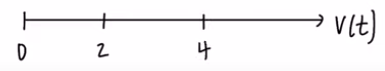
\includegraphics[scale=1]{1.png  }
   \end{center}
   \bigbreak \noindent 
   To start we will test the interval 0-2, so if we plug in 1 into (t-2)(t-4), we get
   a negative times a negative, which will be a \textbf{\textit{\underline{positive}}},
   therefore the velocity in this interval is positive

   \bigbreak \noindent 
   Now if we test the interval 2-4, with 3, we will get a negative times a positive, which is \textbf{\textit{\underline{negative}}}, therefore the 
   velocity in the this interval is negative

   \bigbreak \noindent 
   Last if we test the interval for 4 onward, with 5, we will get a positive times a positive, so the velocity in this 
   interval is positive.

   \bigbreak \noindent 
   \textbf{\textit{\underline{Therefore:}}}
   \bigbreak \noindent 
   \textbf{The particle is moving in the positive direction in the intervals:}
     \begin{align*}
       [0,2)\cup(4,\infty]
     .\end{align*}

   \bigbreak \noindent 
   \nt{Since $v(0) = 24>0$, we will include zero on the interval, also notice the 2 and 4 is not inclusive}

   \bigbreak \noindent 
   \textbf{d.) What is the total distance traveled during the first 6 seconds?}

   \bigbreak \noindent 
   \textit{In order to compute the total distance traveled:}
   \begin{align*}
     total\ distance\ = \abs{f(2)-f(0)} + \abs{f(4)- f(2)} + \abs{f(6)-f(4)}
   .\end{align*}
   \bigbreak \noindent
   \textit{So:}
   \begin{align*}
     \abs{20-0}+ \abs{16-20}+ \abs{36-16} \\
     = 20 + 4 + 20 \\
     = 44\ ft
   \end{align*}

   \bigbreak \noindent 
   \textbf{\textit{\underline{Extra:}}}
   \begin{align*}
     displacement\ = f(6) - f(0) \\
     = 36-0 \\
     = 36ft
   .\end{align*}

   \bigbreak \noindent 
   \textbf{e.) what is the acceleration of the particle at time t?}

   \bigbreak \noindent 
   \textit{to find this, we must find the second derivative of the velocity function}
   \bigbreak \noindent
   \textit{So:}
   \begin{align*}
     a(t) = 6t-18
   \end{align*}

   \bigbreak \noindent 
   \textbf{f.) When is the particle speeding up, and when is it slowing down?}

   \bigbreak \noindent 
   \textit{It is speeding up when v(t) and a(t) have the same sign, and it is slowing 
     down when v(t) and a(t) have opposite signs
   }
   
   \bigbreak \noindent 
   \textit{we will use the number line again, and then make a new one for a(t):}

   \bigbreak \noindent 
   \begin{center}
     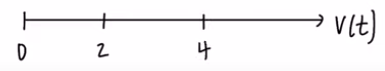
\includegraphics[scale=1]{1.png}
   \end{center}

   \bigbreak \noindent 
   \textit{to construct the number line of a(t), we need to set a(t) = 0 }
   \begin{align*}
    6t-18 = 0 \\
    t = 3
   .\end{align*}
   \bigbreak \noindent 
   \begin{center}
     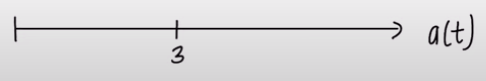
\includegraphics[scale=0.8]{2.png}
   \end{center}

   \bigbreak \noindent 
   so if we plug in something smaller than 3, say \textbf{2}, then:
   \begin{align*}
     6(2) - 18 \\ 
     = -6
   .\end{align*}
   \bigbreak \noindent 
   And if we plug in something bigger than 3, say 4, then:
   \begin{align*}
     6(4) - 18 \\
     =6
   .\end{align*}
   \bigbreak \noindent 
   So smaller than 3 is negative and bigger than 3 is positive.

   \bigbreak \noindent 
   Now if we stack our 2 number lines, and draw lines through each of the zeros,
   we can find when the signs are the same, and when they are opposite to determine
   when the particle is speeding up and slowing down. 

   \bigbreak \noindent
   \textit{So:}
   \begin{center}
     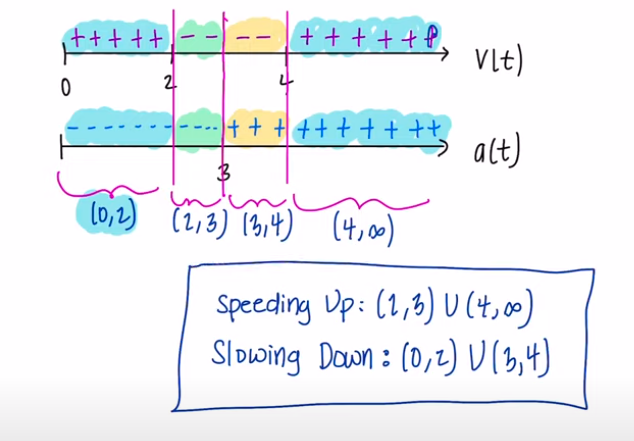
\includegraphics[scale=0.8]{3.png}
   \end{center}

   \pagebreak 
   \begin{mdframed}
     \textbf{\textit{\underline{Example:}}} \textbf{The height (in meters) of a projectile shot vertically upward
       from a point 3 feet above ground level with an initial velocity of $40ft\diagdown s$ is $h=3+40t-16t^{2}$
     }
     \bigbreak \noindent 
     \textbf{a.) Find the velocity after 2 seconds and after 4 seconds}
     \smallbreak \noindent
     \textbf{b.) When does the projectile reach its maximum height?}
     \smallbreak \noindent
     \textbf{c.) What is the maximum height?}
     \smallbreak \noindent
     \textbf{d.) When does it hit the ground?}
     \smallbreak \noindent
     \textbf{e.) With what velocity does it hit the ground?}
   \end{mdframed}

   \bigbreak \noindent 
   \textbf{a.) To get v(t), take the derivative of h and plug in values 2 and 4:}
   \begin{align*}
     v(t) = h^{\prime}(t) = 40-32t
   .\end{align*}
   \begin{align*}
     v(2) = 40-64 \\
     = -24 ft\diagdown s
   .\end{align*}
   \begin{align*}
     v(4) = 40 - 128 \\
     = -88 ft\diagdown s
   .\end{align*}

   \bigbreak \noindent
   \textbf{b.) Set v(t) =  0}
   \begin{align*}
     40 - 32t = 0 \\
     t = \frac{40}{32} \\
     = \frac{4}{5}\ seconds
   .\end{align*}

   \bigbreak \noindent 
   \nt{we set the velocity function equal to zero, because when the projectile reaches
     its max height, it will stop moving before the velocity changes to negative
   }

   \bigbreak \noindent 
   \textbf{c.) Plug $\frac{5}{4}$ into h from the original equation:}
   \begin{align*}
     h(\frac{5}{4}) = 3+40(\frac{5}{4}) - 16(\frac{5}{4})^{2} \\
     = 28ft
   .\end{align*}

   \bigbreak \noindent 
   \textbf{d.) Set h equal to zero and solve:}
   \begin{align*}
     3+40t-16t^{2} =  0 \\
     = 16t^{2} -40t -3
   .\end{align*}
    \textit{Since this will not factor, we must use the quadratic formula:}
    \bigbreak \noindent 
    \textbf{If:}
    \begin{align*}
     \frac{-b\pm \sqrt{b^{2}-4ac}}{2a} 
    .\end{align*}
    \bigbreak \noindent 
    \textit{And:}
    \begin{align*}
      a = 16 \\
      b = -40 \\
      c = -3
    .\end{align*}
    \bigbreak \noindent 
    \textit{Then:}
    \begin{align*}
      t = \frac{40\pm \sqrt{40^{2}-4(16)(-3)}}{2(16)} \\
      t = \frac{40 \pm \sqrt{1792}}{32} \\ 
      t = \frac{40 \pm 16\sqrt{7}}{32} \\
      t = \frac{5 \pm 2\sqrt{7}}{4}
    .\end{align*}

    \bigbreak \noindent 
    \textit{Since we are dealing with time, we will only report the positive value}

    \bigbreak \noindent
    \textit{So:}
    \begin{align*}
      \frac{5 + 2 \sqrt{7}}{4}\ seconds
    \end{align*}

    \bigbreak \noindent 
    \textbf{e.) Plug what we found for t into the velocity function:}
    \begin{align*}
      v(\frac{5+2\sqrt{7}}{4}) = 40-32(\frac{5+2\sqrt{7}}{4}) \\
      = 40 - 40-16\sqrt{7} \\
      = -16\sqrt{7} ft\diagdown s
    .\end{align*}

    \bigbreak \noindent 
    \begin{mdframed}
      \textbf{\textit{\underline{Example:}}} if a rock is thrown vertically upward from the surface of Mars 
      with a velocity of $15 m \diagdown s$, then its height after $t$ seconds is $h = 15t - 1.86t^{2}$
       \bigbreak \noindent 
       \textbf{a.) What is the velocity of the rock after 2 seconds?}
       \smallbreak \noindent
       \textbf{b.) What is the velocity of the rock when its height is 25m on its way up? On its way down?}
    \end{mdframed}

    \bigbreak \noindent 
    \textbf{a.) Find the derivitate of h and plug in 2}
    \bigbreak \noindent
    \textit{So:}
    \begin{align*}
      v(t) = h^{\prime} = 15 - 3.72t
    \end{align*}
    \begin{align*}
      v(2)=  15 - 3.72(2) \\ 
      = 7.56 m \diagdown s
    .\end{align*}

    \bigbreak \noindent 
    \textbf{b.) Set h(t) = 25} 

    \bigbreak \noindent 
    \textit{Graph to visualize:}
    \begin{center}
      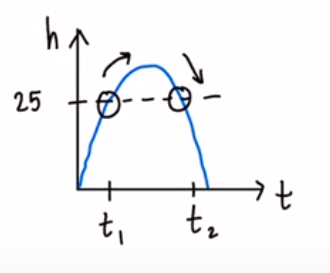
\includegraphics[scale=0.8]{4.png}
    \end{center}

    \bigbreak \noindent
    \textit{So:}
    \begin{align*}
      25 = 15t-1.86t^{2} \\ 
      = 1.86t^{2} -15t -25
    \end{align*}

    \bigbreak \noindent 
    \textit{Now we will use the quadratic formula}
    \begin{align*}
      t = \frac{15\pm \sqrt{225 - 4(1.86)(25)}}{2(1.86)} \\
      = \frac{15\pm \sqrt{225-186}}{3.72} \\
      =  \frac{15\pm \sqrt{39}}{3.72} 
      \approx 5.71, 2.35
    .\end{align*}
      
    \bigbreak \noindent 
    \nt{The earlier time is on the way up, and the later time is on the way down.}

    \bigbreak \noindent 
    \textit{From here we need to find the velocity at each of these times, so we plug them both into the velocity function:}
    \begin{align*}
      v(2.35) = 15-3.72(2.35) \\
      \approx 6.26 m \diagdown s 
    .\end{align*}
    \begin{align*}
      v(5.71) = 15-3.72(5.71) \\
      \approx - 6.24 m \diagdown s 
    .\end{align*}

    \bigbreak \noindent 
    \textbf{\textit{\underline{Summerize:}}}
    \begin{center}
      $s(t)$  $\longrightarrow$ position fxn, also sometimes ($h(t), x(t), y(t), f(t)\ etc...$) 
      \smallbreak \noindent
      $s^{\prime}(t) = v(t)\ (velocity\ function)$ 
      \smallbreak \noindent
      $s^{\prime\prime}(t) = v^{\prime}(t) = a(t)\ (acceleration\ function)$
    \end{center}

    \pagebreak \bigbreak \noindent
    \begin{Large}
        \begin{mdframed}
            \begin{center}
                \textbf{3.8}
            \end{center}
        \end{mdframed}
    \end{Large}
    \begin{Large}
        \begin{center}
            \textbf{Exponential Growth and Decay}
        \end{center}
    \end{Large}
    \line(1,0){490}
    
    \bigbreak \noindent
    In many situations, quantities grow at a rate proportional to their size.
    This quantity can represent a population of people, or a bacteria culture,
    or many other things. In this case, if $y$ is the amount at time  $t$, and we 
    know the rate of change of $y$ is proportional to $y$, then we say:
     \begin{align*}
      \frac{dy}{dt} = ky
    .\end{align*}
    \bigbreak \noindent 
    This differential equation is called the \textbf{\textit{\underline{law of natural growth (or decay)}}}
    and the value of $k$ is called the relative growth rate.
    \begin{align*}
      \frac{1}{y} \cdot \frac{dy}{dt} = k 
    .\end{align*}
    \textit{Where:}
    \begin{align*}
      y = population \\
      \frac{dy}{dt} = growth\ rate
    .\end{align*}
    \bigbreak \noindent 
    \textit{So we can see that:}
    \begin{align*}
        k = \frac{growth\ rate}{population} 
    .\end{align*}
    \bigbreak \noindent 
    \textit{And k is a percent rate of growth:}
    \bigbreak \noindent 
    \textit{If:}
    \begin{align*}
      k = 0.03
    .\end{align*}
    \bigbreak \noindent 
    \textit{Then we have a relative growth rate of 3\%}
    
    \bigbreak \noindent 
    \textbf{\textit{\underline{So do we know a function that would satisfy this equation?}}}
    \begin{align*}
      y = Ce^{kt}
    .\end{align*}
    \bigbreak \noindent 
    \textit{If we derive this equation:}
    \begin{align*}
      \frac{dy}{dt} = C \cdot e^{kt} \cdot  k \\ 
      = k \cdot Ce^{kt}
    .\end{align*}
    \bigbreak \noindent 
    \textit{And we know $y = Ce^{kt}$, Therefore:}
    \begin{align*}
      \frac{dy}{dt} = k \cdot y
    .\end{align*}
    \bigbreak \noindent 
    \nt{If t = 0, then $y = Ce^{0} = c $, so C is the INITIAL VALUE}

    \pagebreak 
    \begin{mdframed}
      \textbf{\textit{\underline{Example:}}} \textbf{A bacterial culture starts with 4000 bacteria and triples every half hour.}
      \bigbreak \noindent 
      \textbf{a.) Find an expression for the number of bacteria after $t$ hours.}
      \smallbreak \noindent
      \textbf{b.) Find the number of bacteria after 20 minutes}
      \smallbreak \noindent
      \textbf{c.) When will the population reach 20,000?}
    \end{mdframed}

    \bigbreak \noindent 
    \textbf{a.)}
    \begin{align*}
      y = Ce^{kt}, c = 4000 \\ 
    .\end{align*}
    \bigbreak \noindent 
    \textit{We know that the value tripes in a half hour, so:}
    \begin{align*}
      (\frac{1}{2}, 12000)      
    .\end{align*}
    \bigbreak \noindent 
    \textit{as (t, y)}
    \begin{align*}
      y = 4000e^{kt}
    .\end{align*}
    \bigbreak \noindent 
    \textit{Now we can plug $(\frac{1}{2},12000)$} into our equation to find k:
    \begin{align*}
      12000 = 4000e^{k \cdot \frac{1}{2}} \\
      = 3 = e^{\frac{k}{2}} \\
      \ln{3}  = \frac{k}{2} \\
      k  = 2\ln{3}  \\
      \approx 2.1972
    .\end{align*}
    \bigbreak \noindent 
    \textit{Now that we found $k$, we can plug it into our equation:}
    \begin{align*}
      y=  4000e^{2.1972 t}
    .\end{align*}
    \bigbreak \noindent 
    \textbf{\textit{\underline{Or:}}}
    \begin{align*}
      y = 4000 \cdot e^{2\ln{3}\cdot t} \\ 
      = 4000 \cdot e^{\ln{9} \cdot t} \\ 
      = y = 4000(9)t
    .\end{align*}

    \bigbreak \noindent 
    \textbf{b.)}
    \begin{align*}
      t = \frac{1}{3}     
    .\end{align*}
    \bigbreak \noindent
    \textit{So:}
    \begin{align*}
      y(\frac{1}{3}) = 4000e^{2.1972(\frac{1}{3})} \\
      \approx 8320\ bacteria
    .\end{align*}
    \bigbreak \noindent 
    \textbf{\textit{\underline{Or:}}}
    \begin{align*}
      y = 4000 \cdot 9^{\frac{1}{3}} \\
      \approx 8320\ bacteria 
    .\end{align*}

    \bigbreak \noindent 
    \textbf{c.) Set y = 20000 (we will use second model)}
    \begin{align*}
      20000 = 4000 \cdot 9^{t} \\ 
      5=  9^{t} \\ 
      = \ln{5} = \ln{9^{t}} \\
      = \ln{5} = t \cdot \ln{9} \\
      t = \frac{\ln{5}}{\ln{9}} \\
      \approx 0.7325\ hrs
    .\end{align*}

    \bigbreak \noindent 
    \begin{mdframed}
      \textbf{As you have probably previously seen, similar exponential functions can be used to 
        represent radioactive decay. In this case the value of $k$ will turn
        out to be negative. The term half-life is used to describe the amount of time
        it takes for half of any given amount to decay away.
      }
      \bigbreak \noindent 
      \textbf{\textit{\underline{Example:}}} \textbf{Polonium-210 has a half-life of 140 days.}
      \bigbreak \noindent 
      \textbf{a.) If a sample has a mass of 200mg, find a formula for the mass that
        remains after $t$ days.
      }
      \smallbreak \noindent
      \textbf{b.) Find the mass after 100 days.}
      \smallbreak \noindent
      \textbf{c.) When will the mass be reduced to 10mg?}
    \end{mdframed}

    \bigbreak \noindent 
    \textbf{a.)}
    \bigbreak \noindent 
    \textit{If:}
    \begin{align*}
      y  = Ce^{kt} 
    .\end{align*}
    \bigbreak \noindent 
    \textit{And:}
    \begin{align*}
      C = 200
    .\end{align*}
    \textit{And:}
    \begin{align*}
      (140, 100)
    .\end{align*}
    \textit{as (t,y)}
    \begin{align*}
      100 = 200e^{k \cdot 140} \\
      \frac{1}{2} = e^{140k} \\
      \ln{\frac{1}{2}} = 140k \\
      k = \frac{\ln{\frac{1}{2}}}{140} \\
      \approx -0.004951
    .\end{align*}
    \bigbreak \noindent
    \textit{So:}
    \begin{align*}
      y = 200e^{-0.004951t}
    \end{align*}

    \bigbreak \noindent 
    \textbf{b.)}
    \begin{align*}
      y(100) = 200e^{-0.004951(100)} \\
      \approx 122
    .\end{align*}

    \bigbreak \noindent 
    \textbf{c.)}
    \begin{align*}
      10 = 200e^{-0.004951t} \\ 
      0.05 = e^{-0.004951t} \\
      \ln{0.05} = -0.004951t \\
      t = \frac{\ln{0.05}}{-0.004951} \\
      \approx 605 days
    .\end{align*}

    \bigbreak \noindent 
    \begin{mdframed}
      \textbf{Next, let's consider an application you may have not encountered before:
        Newton's law of cooling.
      }
      \smallbreak \noindent
      \textbf{Newton's law of cooling says that the rate of cooling of an object is proportional to the temperature 
      difference between the object and its surroundings (if the difference is not too large)}
      \bigbreak \noindent 
      \textbf{\textit{\underline{Newton's law of cooling:}}}
      \begin{align*}
        T(t) = t_s + Ce^{kt}
      .\end{align*}
      \bigbreak \noindent 
      \textit{Where $T(t)$ is the temperature of object at time  $t$, and $t_s$ is the temperature of surroundings}
      \smallbreak \noindent
      \textit{And:}
      \begin{align*}
        C = t_0 - t_s
      .\end{align*}
    \end{mdframed}

    \bigbreak \noindent 
    \begin{mdframed}
      \textbf{\textit{\underline{Example:}}} \textbf{A freshly brewed cup of coffee has a temperature of
      $95^{\circ}$C in a $20^{\circ}$C room, five minutes later, its temerature is $88^{\circ}C$
      }
      \bigbreak \noindent 
      \textbf{a.) find a function that gives the temperature reading after $t$ minutes.}
      \smallbreak \noindent
      \textbf{b.) What is the temperature reading after 10 minutes?}
      \smallbreak \noindent
      \textbf{c.) When will the temperature reading be $70^{\circ}C$?}
    \end{mdframed}

    \bigbreak \noindent 
    \textbf{a.)}
    \begin{align*}
      C = t_0 - t_s  = 95-20 \\
      = 75
    .\end{align*}
    \bigbreak \noindent
    \textit{So:}
    \begin{align*}
      T(t) = 20 + 75e^{kt}
    \end{align*}
    \bigbreak \noindent 
    \textit{And:}
    \begin{align*}
      (5, 88)
    .\end{align*}
    \bigbreak \noindent 
    \textit{As (T(t), t):}
    \bigbreak \noindent
    \textit{So:}
    \begin{align*}
      88 = 20 + 75e^{k \cdot 5} \\
      68 = 75e^{5k} \\ 
      \frac{68}{75} = e^{5k} \\
      \ln{\frac{68}{75}} = 5k \\
      k = \frac{\ln{\frac{68}{75}}}{5} \\
      \approx -0.0196
    \end{align*}

    \bigbreak \noindent 
    \textit{Now:}
    \begin{align*}
      T(t) = 20 + 75e^{-0.0196t}
    .\end{align*}

    \bigbreak \noindent
    \textbf{b.)}
    \begin{align*}
      T(t) = 20 + 75e^{-0.0196(10)} \\ 
      \approx 81.78^{\circ}C
    .\end{align*}

    \bigbreak \noindent 
    \textbf{c.)}
    \begin{align*}
      70 = 20 + 75e^{-0.0196t} \\
      50 = 75e^{-0.0196t} \\
      \frac{2}{3} = e^{-0.0196t} \\
      \ln{\frac{2}{3}} = -0.0196t \\
      t = \frac{\ln{\frac{2}{3}}}{-0.0196} \\
      \approx 20.71\ min
    .\end{align*}

    \bigbreak \noindent 
    \begin{mdframed}
      \textbf{\textit{\underline{Example:}}} \textbf{A thermometer in air-conditioned room
        reads $70^{\circ}F$. The thermometer is taken outdoors where the temperature is $92^{\circ}f$.
        After 1 minute the thermometer reads $81^{\circ}F$. What is the reading after 2 minutes? When will
        the thermometer read $90^{\circ}F$?
      }
    \end{mdframed}
    \bigbreak \noindent
    \textit{So:}
    \begin{align*}
      C =  t_0 - t_s = 70-92\\
      = -22
    \end{align*}
    \bigbreak \noindent 
    \textit{And:}
    \begin{align*}
      (81,1)
    .\end{align*}
    \bigbreak \noindent 
    \textit{As (T(t), t)}
    \bigbreak \noindent
    \textit{So:}
    \begin{align*}
      T(t) = 92 - 22e^{kt}      
    \end{align*}
    \begin{align*}
      81 = 92-22e^{k(1)} \\
      \frac{11}{22} = e^{k} \\
      k = \ln{\frac{11}{22}} \\
      k \approx -0.6931
    .\end{align*}

    \bigbreak \noindent 
    \textit{Therefore:}
    \begin{align*}
      T(t) = 92 -22e^{-0.6931t}
    .\end{align*}

    \bigbreak \noindent 
    \textit{Now plug in 2 for t:}
    \begin{align*}
      T(t) = 92-22e^{-0.6931(2)} \\
      \approx 86^{\circ}F
    .\end{align*}

    \bigbreak \noindent 
    \textit{Last:}
    \begin{align*}
      90 = 92- 22e^{-0.6931t} \\ 
      -\frac{2}{22} = e^{-0.6931t} \\
      \frac{1}{11} = e^{-0.6931t} \\
      \ln{\frac{1}{11}} = -0.6931t \\
      t = \frac{\ln{\frac{1}{11}}}{-0.6931} \\
      t  \approx 3.5\ min
    .\end{align*}

    \pagebreak \bigbreak \noindent
    \begin{Large}
        \begin{mdframed}
            \begin{center}
                \textbf{3.9}
            \end{center}
        \end{mdframed}
    \end{Large}
    \begin{Large}
        \begin{center}
            \textbf{Related Rates}
        \end{center}
    \end{Large}
    \line(1,0){490}
    
    \bigbreak \noindent 
    Many things change with item. Our goal is to find the rate at which some 
    quantity is changing by relating it to other quantities whose rates of 
    change are given or more easily measured 

    \bigbreak \noindent 
    \textbf{Strategy}
    \begin{enumerate}
      \item Read the problem carefully
      \item Draw a diagram whenever possible
      \item Introduce notation
      \item Express rates in terms of derivatives
      \item Write an equation 
      \item Differentiate both sides with repect to $t$ using Implicit Differentiation/Chain Rule
      \item Solve for the unknown rate
    \end{enumerate}

    \bigbreak \noindent 
    \begin{mdframed}
      \textbf{Example:}
      The length of a rectangle is increasing at a rate of 8 cm/s and it's
      width is increasing at a rate of 3 cm/s. When the length is 20cm and the
      width is 10cm, how fast is the area increasing?
    \end{mdframed}
    \bigbreak \noindent
    \textit{So:}
    \begin{align*}
      \frac{dt}{dl} = 8cm \diagdown s
    \end{align*}
    \bigbreak \noindent 
    \textit{And:}
    \begin{align*}
      \frac{dw}{dt} = 3cm \diagdown s
    .\end{align*}

    \bigbreak \noindent 
    \textit{We want:}
    \begin{align*}
      \frac{da}{dt}
    .\end{align*}
    \bigbreak \noindent 
    \textit{When:}
    \begin{align*}
      l = 20cm \\ 
      w = 10cm
    .\end{align*}

    \bigbreak \noindent 
    \textit{We will use the area formula and take the deriviative of both sides:}
    \begin{align*}
      \frac{d}{dt} A = \frac{d}{dt}(l \cdot w)
    .\end{align*}

    \bigbreak \noindent 
    \textit{We must use the product rule for $l \cdot w$:}
    \begin{align*}
      \frac{da}{dt} = l \cdot \frac{dw}{dt} + \frac{dl}{dt} \cdot w
    .\end{align*}

    \bigbreak \noindent 
    \textit{Now we can plug in values that were given to us:}
    \begin{align*}
      \frac{da}{dt} = (20)(3) + (8)(10) \\ 
      = 60 + 80 \\ 
      = 140\ cm^{2} \diagdown s
    .\end{align*}

    \pagebreak \bigbreak \noindent
    \begin{mdframed}
      \textbf{Example:}
      \begin{align*}
        If\ x^{2} + y^{2} = 25\ and\ \frac{dy}{dt} = 6,\ find\ \frac{dx}{dt}\ when\ y = 4
      .\end{align*}
    \end{mdframed}
    \bigbreak \noindent
    \textit{So:}
    \begin{align*}
      \frac{d}{dt} (x^{2} + y^{2}) = \frac{d}{dt} (25)
    \end{align*}
    \begin{align*}
      2x \cdot \frac{dx}{dt} + 2y \cdot \frac{dy}{dt} = 0 \\ 
      =2x\frac{dx}{dt} = -2y \frac{dy}{dt} \\
      =\frac{dx}{dt} = \frac{-2y \frac{dy}{dt}}{2x} \\
      =\frac{dx}{dt} = \frac{-y \frac{dy}{dt}}{x} \\
    .\end{align*}

    \bigbreak \noindent 
    \textit{From here we can plug in what they gave us, but first we need to find x:}
    \begin{align*}
        x^{2} + 4 = 25 \\
        x^{2} = 9 \\
        x = \pm 3
    .\end{align*}

    \bigbreak \noindent 
    \textit{
      Now:
    }
    \begin{align*}
      if\ x = 3\text{:}\ \frac{dx}{dt} = \frac{(-4)(6)}{3} \\
    = -8
    .\end{align*}
    \begin{align*}
      if\ x = -3\text{:}\ \frac{dx}{dt} = \frac{(-4)(6)}{-3} \\
      = 8
    .\end{align*}

    \bigbreak \noindent 
    \begin{mdframed}
      \textbf{Example:}
      At noon, Ship A is 150km west of ship B. Ship A is sailing east at 35km/h
      and ship B is sailing north at 25km/h. How fast is the distance between the ships
      changing at 4:00 pm? 
    \end{mdframed}
    \bigbreak \noindent
    \textit{So:}
    \begin{center}
      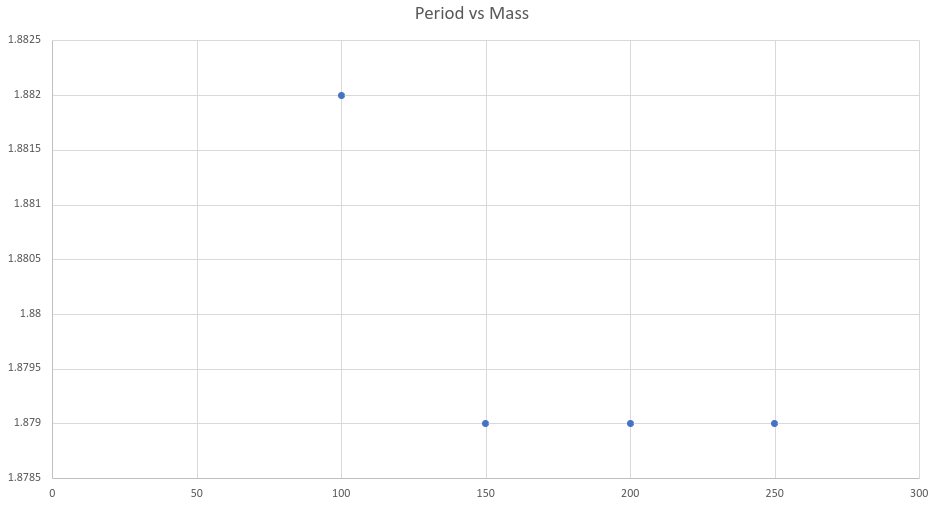
\includegraphics[scale=.6]{ ~/Pictures/1.png }
      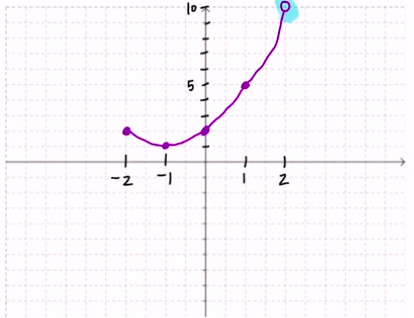
\includegraphics[scale=0.6]{ ~/Pictures/2.png }
    \end{center}

    \bigbreak \noindent 
    \textit{We want: $\frac{dz}{dt}$ at 4pm:}

    \bigbreak \noindent 
    \textit{We know:}
    \begin{align*}
      \frac{dx}{dt} = -35 km \diagdown h
    .\end{align*}
    \begin{align*}
      \frac{dy}{dt} = 25 km \diagdown h
    .\end{align*}
    \bigbreak \noindent 
    \nt{$\frac{dx}{dt}$ is negative because it's moving in a way that's getting closer to where ship B used to be}

    \bigbreak \noindent 
    \textit{Since we have a right triangle we will use the Pythagorean theorem:}
    \begin{align*}
      x^{2} + y^{2} = z^{2}
    .\end{align*}
    \bigbreak \noindent
    \textit{So:}
    \begin{align*}
      \frac{d}{dt}(x^{2}+y^{2}) = \frac{d}{dt}(z^{2}) \\ 
      2x \cdot \frac{dx}{dt}  +2y \frac{dy}{dt} = 2z \cdot \frac{dz}{dt}
    \end{align*}

    \bigbreak \noindent 
    \textit{Cancel out the 2s and find x, y and z at 4pm:}
    \begin{align*}
      x \frac{dx}{dt} + y \frac{dy}{dt} = z \frac{dz}{dt}
    .\end{align*}

    \bigbreak \noindent
    \textit{So:}
    \begin{align*}
      \text{Ship A has traveled $35(4) = 140 km$} \\
      x = 150 - 140 = 10\ km
    \end{align*}
    \begin{align*}
      \text{Ship B has traveled $25(4) = 100\ km$} \\
      y = 100\ km
    .\end{align*}
    \begin{align*}
      10^{2} + 100^{2} = z^{2} \\ 
      z = \sqrt{10,100} \\ 
      = 10\sqrt{101}
    .\end{align*}

    \bigbreak \noindent
    \textit{Now:}
    \begin{align*}
      10(-35) + (100)(25) = 10\sqrt{101} \frac{dz}{dt} \\ 
      \frac{dz}{dt} = \frac{-350 + 2500}{10\sqrt{101}} \\ 
      = \frac{2150}{10\sqrt{101}} \\
      = \frac{215}{\sqrt{101}} \\
      \approx 21.39\ km \diagdown h
    \end{align*}

    \pagebreak \bigbreak \noindent
    \begin{mdframed}
      \textbf{Example:}
      A trough is 10 ft long and it's ends have the shape of isosceles triangles 
      that are 3ft across at the top and have a height of 1 ft. If the trough is 
      being filled with water at a rate of $12ft^{3} \diagdown min$, how fast
      is the water level rising when the water is 6 in. deep? 
    \end{mdframed}

    \bigbreak \noindent 
    \textit{We know:}
    \begin{align*}
      \frac{dv}{dt} = 12 ft^{3} \diagdown min
    .\end{align*}
    \begin{align*}
      let\ h\  = height\ of\ water
    .\end{align*}

    \bigbreak \noindent 
    \begin{center}
      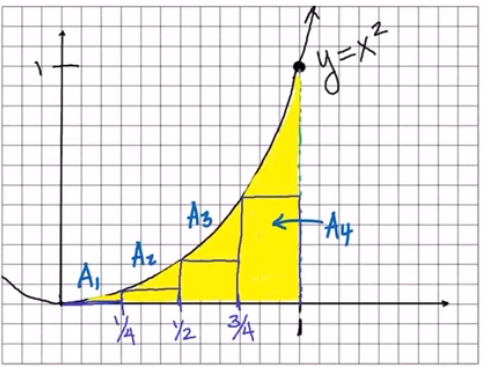
\includegraphics[scale=0.5]{~/Pictures/3.png}
    \end{center}

    \bigbreak \noindent 
    \textit{To get the volumne of the water, it's the area of the small triangle in blue,
      multiplied by 10
     }
     \bigbreak \noindent
     \textit{So:}
     \begin{align*}
       \frac{1}{2}b \cdot h  \cdot 10 \\
       = 5bh
     \end{align*}
  
    \bigbreak \noindent 
    \textit{We need to express b in terms of h because both b and h change as the water rises, so we need to use similar triangles}

    \bigbreak \noindent 
    \begin{center}
      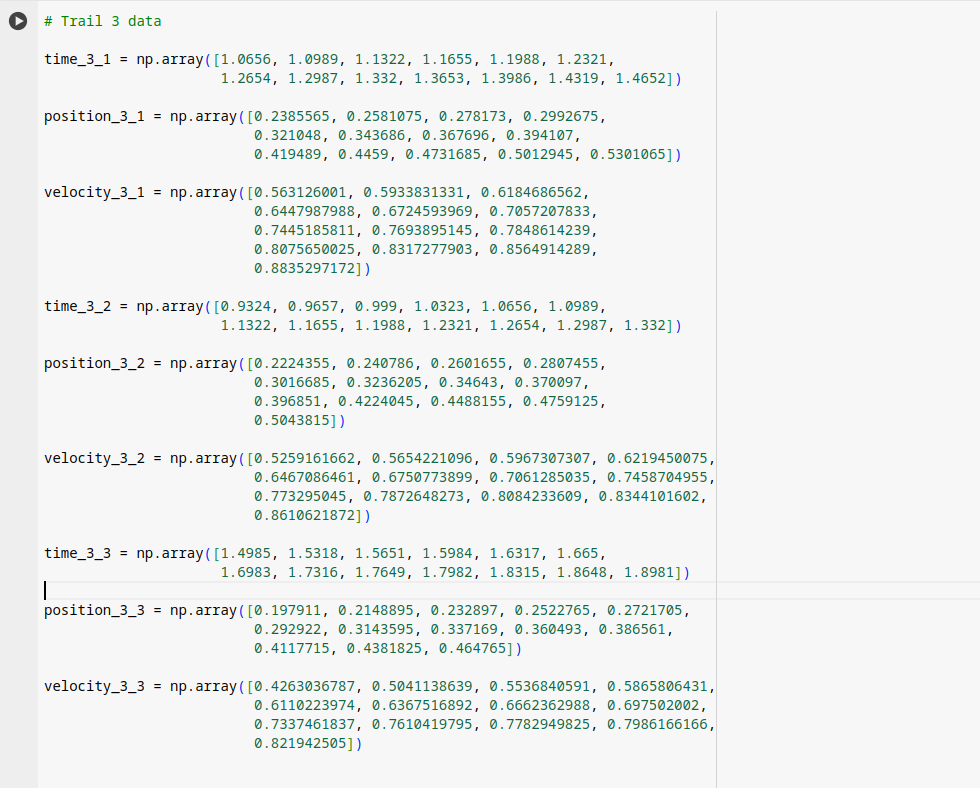
\includegraphics[scale=1]{ ~/Pictures/4.png }
    \end{center}
    \bigbreak \noindent
    \textit{So:}
    \begin{align*}
      \frac{3}{1} = \frac{b}{h} \\ 
      3h = b
    \end{align*}
    \bigbreak \noindent 
    \textit{Now we can put it back into the volumne formula:}
    \begin{align*}
      v = 5bh \\
      = 5(3h)h \\
      v(h) =15h^{2}
    .\end{align*}

    \bigbreak \noindent 
    \textit{Now we can differentiate with respect to t:}
    \begin{align*}
      \frac{dv}{dt} = 30h \cdot \frac{dh}{dt} \\
      12 = 30(0.5) \frac{dh}{dt} \\ 
      \frac{dh}{dt} = \frac{12}{15} \\
      = \frac{4}{5}\ ft \diagdown min
    .\end{align*}

    \pagebreak \bigbreak \noindent
    \begin{Large}
        \begin{mdframed}
            \begin{center}
                \textbf{3.10}
            \end{center}
        \end{mdframed}
    \end{Large}
    \begin{Large}
        \begin{center}
            \textbf{Linear Approximations and Diffentials}
        \end{center}
    \end{Large}
    \line(1,0){490}
    
    \bigbreak \noindent \bigbreak \noindent 
    \begin{center}
      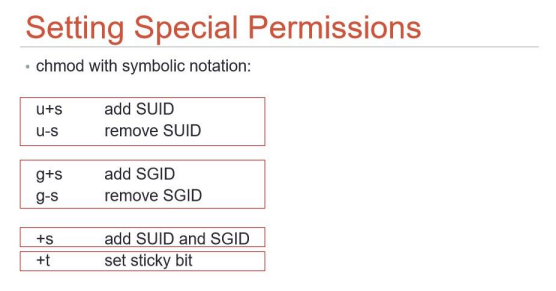
\includegraphics[scale=0.6]{ ~/Pictures/5.png}
    \end{center}
    \bigbreak \noindent 
    Notice, near $x = a$, the values of  $f(x)$ and  $L(x)$ are very close
    to each other. This concept is helpful to approximate values of $f(x)$ near $x=a$ 
    using $L(x)$. This process is called  \textbf{\textit{\underline{Linear Approximation}}} of
    $f(x)$ at $x=a$ 

    \bigbreak \noindent 
    \begin{align*}
      \boxed{f(x) \approx L(x) = f(a) + f^{\prime}(a)(x-a)}
    .\end{align*}

    \bigbreak \noindent 
    \begin{center}
      Slope of $L(x) = f^{\prime}(a)$ at the point (a, f(a)). \\
      The equation of $L(x):$ \\ 
      recall:  $y-y_1 = m(x-x_1)$
    \end{center}

    \bigbreak \noindent 
    \textit{Note that:}
    \begin{align*}
      m\ is\ f^{\prime}(a) \\ 
      (a, f(a))\ is\ (x_1, y_1)
    .\end{align*}

    \bigbreak \noindent 
    \begin{mdframed}
      \textbf{Example: Find the linearization of the function:}
      \begin{align*}
         f(x) = \frac{2}{\sqrt{x^{2} -5}}\ at\ a = 3 
      .\end{align*}
    \end{mdframed}

    \bigbreak \noindent 
    \nt{This means the same thing as "find the equation of the tangent line to the curve". 
      We are just replacing y with $L(x)$
    }

    \bigbreak \noindent
    \textit{So:}
    \begin{align*}
      f(x) =  2(x^{2} - 5)^{-\frac{1}{2}}
    \end{align*}
    \begin{align*}
      f^{\prime}(x) = 2(-\frac{1}{2})(x^{2} -5)^{-\frac{3}{2}} \cdot 2x \\
      = -2x(x^{2} -5)^{-\frac{3}{2}} \\ 
      = \frac{-2x}{(x^{2}-5)^{\frac{3}{2}}}
    .\end{align*}

    \bigbreak \noindent 
    \textit{Now to find slope we plug in 3:}
    \begin{align*}
      m = f^{\prime}(3) = \frac{-2(3)}{(9-5)^{\frac{3}{2}}}  \\
      = -\frac{6}{8} \\ 
      = -\frac{3}{4}
    .\end{align*}

    \bigbreak \noindent 
    \textit{Now we need a point, which is at (a, f(a)):}
    \begin{align*}
      so\ \bigg(3, \frac{2}{\sqrt{9-5}}\bigg) \\
      = (3,1)
    .\end{align*}

    \bigbreak \noindent 
    \textit{Now we use formula from beginning of lession:}
    \begin{align*}
      L(x) = f(3) + f^{\prime}(3)(x-a)
    .\end{align*}
    \begin{align*}
      L(x) = 1 - \frac{3}{4}(x-3) \\
      = -\frac{3}{4}x + \frac{13}{4}
    .\end{align*}

    \bigbreak \noindent 
    \textbf{\textit{\underline{Final Answer:}}}
    \begin{align*}
      f(x) = \frac{2}{\sqrt{x^{2} -5}} \approx L(x) = -\frac{3}{4}x + \frac{13}{4} \\ 
      near\ x = 3
    .\end{align*}

    \bigbreak \noindent 
    \begin{mdframed}
      \textbf{Example: Find the linear Approximation of:}
      \begin{align*}
        g(x) = \sqrt[3]{1+x}\ at\ x=0 
      .\end{align*}
      And use it to approximate
      \begin{align*}
        \sqrt[3]{0.95}\ and\ \sqrt[3]{1.1}
      .\end{align*}
    \end{mdframed}

    \bigbreak \noindent
    \textit{So:}
    \begin{align*}
      g(x) = (1+x)^{\frac{1}{3}}
    \end{align*}
    \begin{align*}
      g^{\prime}(x) = \frac{1}{3}(1+x)^{-\frac{2}{3}} \cdot 1 \\ 
      = \frac{1}{3(1+x)^{\frac{2}{3}}}
    .\end{align*}

    \bigbreak \noindent 
    \textit{Now find m:}
    \begin{align*}
      g^{\prime}(0) = \frac{1}{3(1+0)^{\frac{2}{3}}} \\ 
      = \frac{1}{3}
    .\end{align*}

    \bigbreak \noindent 
    \textit{Now get point (a, f(a)):}
    \begin{align*}
      f(0) = \sqrt[3]{1+0} \\ 
      = 1
    .\end{align*}
    \begin{align*}
      (0,1)
    .\end{align*}

    \bigbreak \noindent 
    \textit{Now plug into linear approximation formula:}
    \begin{align*}
      L(x) = f(a) + f^{\prime}(a)(x-a) \\ 
      = 1 + \frac{1}{3}(x-0) \\ 
      = 1+ \frac{1}{3}x
    .\end{align*}

    \bigbreak \noindent 
    \textit{Now use this to approximate $\sqrt[3]{0.95}\ and\ \sqrt[3]{1.1}$}

    \bigbreak \noindent 
    \textbf{\textit{\underline{$\sqrt[3]{0.95}$}}}

    \bigbreak \noindent 
    \textit{Since:}
    \begin{align*}
      \sqrt[3]{0.95} = \sqrt[3]{1+x} \\ 
      0.95 = 1 + x \\
      x = -0.05
    .\end{align*}
    \bigbreak \noindent
    \textit{So:}
    \begin{align*}
      \sqrt[3]{0.95} \approx L(-0.05) = 1+ \frac{1}{3}(-0.05) \\
      = 0.98\overline{3}
    \end{align*}

    \bigbreak \noindent 
    \textbf{\textit{\underline{$\sqrt[3]{1.1}$}}:}

    \bigbreak \noindent 
    \begin{align*}
      \sqrt[3]{1.1} = \sqrt[3]{1+x} \\ 
      = 1.1 = 1 + x \\ 
      = 0.1
    .\end{align*}

    \bigbreak \noindent
    \textit{So:}
    \begin{align*}
      \sqrt[3]{1.1} \approx L(0.1) = 1+ \frac{1}{3}(0.1) \\ 
      = 1.0\overline{3}
    \end{align*}

    \pagebreak \bigbreak \noindent
    \begin{mdframed}
    \begin{large}
        \begin{center}
            \textbf{Diffentials}
        \end{center}
    \end{large}
    \end{mdframed}
    \line(1,0){490}
    \bigbreak \noindent \bigbreak
    \begin{center}
      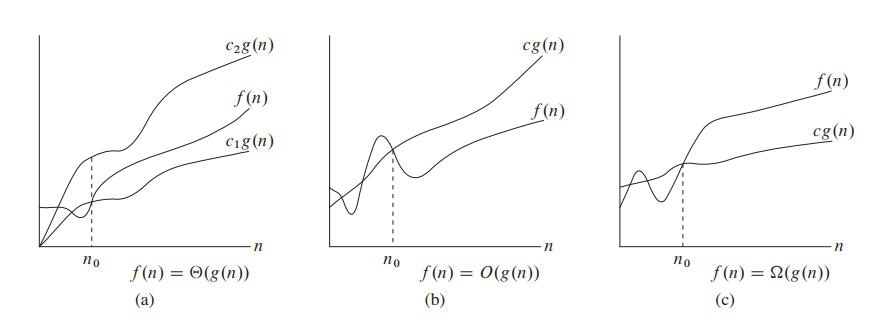
\includegraphics[scale=0.75]{~/Pictures/6.png}
    \end{center}
    \begin{align*}
      m_{tan} = \frac{dy}{dx} \leftarrow \frac{rise}{run}
    .\end{align*}
    \bigbreak \noindent 
    \begin{center}
      Associated with f(x):
    \end{center}
    \begin{align*}
      \triangle x \\
      \triangle y
    .\end{align*}
    \bigbreak \noindent 
    \begin{center}
      Associated with tangent line:
    \end{center}
    \begin{align*}
      dx \\
      dy \\
      f^{\prime}(x) = \frac{dy}{dx}
    .\end{align*}
    \bigbreak \noindent 
    The differential dx is an independent variable.
    \smallbreak \noindent
    The differential dy is defined in terms of dx by:
    \begin{align*}
      \boxed{dy = f^{\prime}(x)dx}
    .\end{align*}
    \bigbreak \noindent 
    How are dy and $\triangle y$ related?
    \begin{itemize}
      \item $\triangle x$ = $dx$
      \item $\triangle y$ represents how much f(x) rises or falls
      \item $dy$ represents how much the tangent line rises or falls
    \end{itemize}
    \begin{align*}
      \boxed{\triangle y  = f(x + \triangle x) -f(x)}
    .\end{align*}
    \begin{center}
      Can be difficult to find, so we use:
    \end{center}
    \begin{align*}
      dy \approx \triangle y
    .\end{align*}

    \pagebreak \bigbreak \noindent
    \begin{mdframed}
      \textbf{Example: Find the differential of:}
      \begin{align*}
        y = \frac{s}{1+2s}
      .\end{align*}
    \end{mdframed}
    \bigbreak \noindent
    \textit{So:}
    \begin{align*}
     dy = f^{\prime}(s)ds 
    \end{align*}

    \bigbreak \noindent 
    \textit{Then by the quotient rule:}
    \begin{align*}
      dy = \frac{(1+2s)(1) - s(2)}{(1+2s)^{2}}ds
    .\end{align*}
    \begin{align*}
      dy = \frac{1+2s - 2s}{(1+2s)^{2}}ds \\
      dy = \frac{1}{(1+2s)^{2}}ds \\
    .\end{align*}

    \bigbreak \noindent 
    \begin{mdframed}
      \textbf{Example: Find the differential of:}
      \begin{align*}
        y = \sqrt{1+\ln{z}}
      .\end{align*}
    \end{mdframed}

    \bigbreak \noindent 
    \textit{By the shortcut:}
    \begin{align*}
      dy = \frac{1}{2\sqrt{1+\ln{z}}} \cdot (\frac{1}{z})dz \\
      = \frac{dz}{2z\sqrt{1+\ln{z}}} \\
    .\end{align*}

    \bigbreak \noindent 
    \begin{mdframed}
      \textbf{Example: Compute $\triangle y$ and $dy$. Then sketch a diagram showing segments with length $dx$, $dy$ 
        and $\triangle y$
      }
      \begin{align*}
        y = \sqrt{x} \\ 
        x =1 \\
        \triangle x = 1
      .\end{align*}
    \end{mdframed}

    \bigbreak \noindent 
    \textit{We know:}
    \begin{align*}
      if\ \triangle x = 1 \\
      dx = 1
    .\end{align*}

    \bigbreak \noindent 
    \textit{Also:}
    \begin{align*}
      y^{\prime} = \frac{1}{2}x^{-\frac{1}{2}}dx
    .\end{align*}

    \bigbreak \noindent 
    \textit{So:}
    \begin{align*}
      dy = f^{\prime}(x)dx
    .\end{align*}

    \bigbreak \noindent 
    \textit{Then:}
    \begin{align*}
      dy = \frac{1}{2} \cdot 1 \cdot 1 \\
      = \frac{1}{2}
    .\end{align*}

    \bigbreak \noindent 
    \textit{And if:}
    \begin{align*}
      \triangle y = f(x + \triangle x) - f(x) \\ 
      = f(1+1) - f(1) \\
      = \sqrt{2} - \sqrt{1} \\
      \approx 0.414
    .\end{align*}

    \bigbreak \noindent 
    \begin{mdframed}
      \textbf{Example: Use a linear approximation of differentials to estimate $e^{-0.015}$}
    \end{mdframed}
    \bigbreak \noindent
    \textit{So:}
    \begin{align*}
      let\ f(x) = e^{x}\ where\ x=-0.015
    \end{align*}

    \bigbreak \noindent 
    \textit{Using differentials, pick a point near -0.015 that we can use as an initial point and we can easily compute:}
    \begin{align*}
      near\ x= 0
    .\end{align*}
    \begin{align*}
      f(x) = e^{x} 
    .\end{align*}
    \begin{align*}
      f^{\prime}(x) = e^{x}
    .\end{align*}
    \begin{align*}
      dy = e^{x}dx
    .\end{align*}
    \begin{align*}
      dx = \triangle x = -0.015
    .\end{align*}
    \begin{align*}
      dy = e^{0} (-0.015) \\
      = -0.015
    .\end{align*}

    \bigbreak \noindent 
    \textit{Now:}
    \begin{align*}
      e^{-0.015} = e^{0} + \triangle y \approx e^{0} + dy \\
      = 1 + (-0.015) \\
      = 1-0.015 \\
      = .985
    .\end{align*}

    \bigbreak \noindent 
    \textit{Using linear application, find $L(x)$ at $a = 0$:}
    \begin{align*}
      f(x) = e^{x}
    .\end{align*}

    \bigbreak \noindent 
    \textit{Recall:}
    \begin{align*}
      L(x) = f(a) + f^{\prime}(a)(x-a)
    .\end{align*}
    \bigbreak \noindent
    \textit{So:}
    \begin{align*}
      f(0) = e^{0} \\
      = 1
    \end{align*}
    \begin{align*}
      m = f^{\prime}(0) = e^{0} \\
      = 1
    .\end{align*}
    \begin{align*}
      (a,f(a)) \\
      = \\
      (0, 1)
    .\end{align*}
    \begin{align*}
      L(x) = 1 + 1(x- 0) \\ 
      = 1+x
    .\end{align*}

    \bigbreak \noindent 
    \textit{Now: }
    \begin{align*}
      e^{-0.015} \approx L(-0.015) \\
      = 1+(-0.015) \\
      = 0.985
    .\end{align*}







  
\end{document}
